\documentclass[preprint,12pt]{elsarticle}

\usepackage{amsmath,amssymb}
\usepackage{graphicx}
\usepackage{booktabs}
\usepackage{hyperref}
\usepackage{natbib}
\usepackage{lineno}
\usepackage{siunitx}
\usepackage{xcolor}

\usepackage{fancyhdr}
\fancypagestyle{preprint}{%
  \fancyhf{}%
  \fancyhead[C]{\small\textit{Non-peer reviewed preprint submitted to EarthArXiv}}%
  \fancyfoot[C]{\thepage}%
  \renewcommand{\headrulewidth}{0pt}%
}
\pagestyle{preprint}

\modulolinenumbers[5]
\journal{EarthArXiv preprint}

\begin{document}

%% ============================================================
%% EARTHARXIV COVERSHEET (page 1)
%% ============================================================
\thispagestyle{empty}
\begin{center}
\vspace*{3cm}

{\LARGE\bfseries Urban Green Cover and Land Surface Temperature in Ho Chi Minh City: A Remote Sensing Analysis of Vegetation Cooling Effects Across Historical Development Rings, 1990--2025}

\vspace{2cm}

{\Large Tue Le-Quang}\\[0.5em]
{\large Urban Social Economics Research Group\\
Fulbright University Vietnam, Ho Chi Minh City, Vietnam}\\[1em]
{\large Email: lqtuevn@gmail.com}\\[0.5em]
{\large ORCID: \url{https://orcid.org/0009-0006-5863-6011}}

\vspace{3cm}

\fbox{\parbox{0.85\textwidth}{\centering\large
This is a non-peer reviewed preprint submitted to \textbf{EarthArXiv}.\\[0.5em]
This preprint has not been submitted to a journal for peer review.
}}

\vspace{2cm}

{\large March 2026}

\end{center}
\clearpage

%% ============================================================
%% MANUSCRIPT
%% ============================================================

\begin{frontmatter}

\title{Urban Green Cover and Land Surface Temperature in Ho Chi Minh City: A Remote Sensing Analysis of Vegetation Cooling Effects Across Historical Development Rings, 1990--2025}

\author[fulbright]{Tue Le-Quang\fnref{orcid}}
\ead{lqtuevn@gmail.com}
\fntext[orcid]{ORCID: \url{https://orcid.org/0009-0006-5863-6011}}

\address[fulbright]{Urban Social Economics Research Group, Fulbright University Vietnam, Ho Chi Minh City, Vietnam}

\begin{abstract}
Urban heat islands pose escalating risks to tropical megacities, yet spatially explicit analyses linking vegetation loss to surface warming remain scarce for Southeast Asian cities with complex colonial and post-war development histories. This study quantifies the relationship between fractional vegetation cover (FVC) and land surface temperature (LST) across Ho Chi Minh City (HCMC) using Sentinel-2 (10\,m) and Landsat 8/9 thermal (100\,m) imagery from 2024--2025, and tracks green cover change across five historical development rings from 1990 to 2020 using the Landsat archive. Regressing LST against FVC for 196,438 pixels at 100\,m resolution yields a significant negative linear relationship ($\text{LST} = 38.15 - 4.95 \times \text{FVC}$, $R^2 = 0.207$), with a quadratic model explaining additional variance ($R^2 = 0.266$). Dense vegetation ($\text{FVC} > 0.90$) is \SI{4.07}{\degreeCelsius} cooler than built-up surfaces ($\text{FVC} < 0.05$). The temporal analysis reveals that HCMC lost approximately 130\,km$^2$ of green area between 2000 and 2020, with the sharpest losses in the 1976--2000 industrial ring ($-18$ percentage points) and the 1972--1976 war-era ring ($-18$ pp). Stratifying HCMC's 113 wards by historical development era shows that the two innermost rings---home to 4.3 million residents---exhibit the lowest vegetation cover (median 8.7--11.3\%) and highest peak surface temperatures (40--42\,\si{\degreeCelsius} in 2015). Thirty-six wards forming a contiguous concrete belt fall below 20\,m$^2$/person of accessible canopy cover, affecting 3.5 million residents. Three wards fail the WHO minimum even within a 1\,km walking buffer, trapping 327,000 residents in green deserts. The results demonstrate that HCMC's urban heat burden is spatially structured by historical planning regimes, and that targeted revegetation of the concrete belt could yield measurable cooling.
\end{abstract}

\begin{keyword}
urban heat island \sep land surface temperature \sep NDVI \sep fractional vegetation cover \sep Ho Chi Minh City \sep Sentinel-2 \sep Landsat \sep green space accessibility \sep urban green space \sep temporal analysis
\end{keyword}

\end{frontmatter}

\linenumbers

%% ============================================================
\section{Introduction}
\label{sec:intro}
%% ============================================================

The urban heat island (UHI) effect---the phenomenon whereby built-up areas exhibit elevated surface and air temperatures relative to surrounding rural land---is among the most well-documented consequences of urbanization \citep{oke1982,arnfield2003}. In tropical megacities, where baseline temperatures already approach human physiological limits, the UHI intensifies heat-related morbidity and mortality, increases cooling energy demand, and degrades outdoor thermal comfort \citep{tan2010,mora2017}.

Vegetation mitigates urban heating through evapotranspiration and shading, producing a measurable negative correlation between the Normalized Difference Vegetation Index (NDVI) and land surface temperature (LST) that has been demonstrated across climatic zones \citep{weng2004,yuan2007,li2013}. \citet{weng2004} established the linear LST--NDVI framework for UHI analysis using Landsat ETM+ over Indianapolis, finding that NDVI explained 42\% of LST variance. Subsequent work confirmed this relationship in tropical Asian cities including Bangkok, Jakarta, and Hanoi \citep{estoque2017,hua2021}, though $R^2$ values typically range from 0.15 to 0.45 depending on spatial resolution, land cover heterogeneity, and acquisition timing.

Ho Chi Minh City (HCMC), Vietnam's largest metropolis with 11.3 million urban residents as of 2025, presents a distinctive case for LST--vegetation analysis. The city's built environment was shaped by four successive political regimes---French colonial (pre-1954), wartime (1954--1975), post-reunification socialist (1975--2000), and market-era development (2000--present)---each of which imprinted a different spatial logic of density, infrastructure, and green space provision on the urban fabric \citep{waibel2006}. The result is a city where vegetation cover varies by an order of magnitude across wards located only kilometers apart, and where the thermal consequences of historical planning decisions are etched into the satellite record.

Despite rapid urbanization and mounting heat stress, spatially explicit LST--vegetation analyses for HCMC remain limited. \citet{tran2017} examined land use--LST relationships in the HCMC region using Landsat but at coarser spatial and thematic resolution. The 2025 administrative restructuring---which merged Vietnam's pre-existing urban wards (\textit{phường}) and rural communes (\textit{xã}) into 687 new urban wards---provides both an opportunity and a methodological challenge, as 53\% of new wards absorbed rural land that inflates aggregate green metrics.

This study makes four contributions. First, the LST--FVC relationship is quantified at 100\,m resolution across the pre-merger HCMC boundary using 2024--2025 Sentinel-2 and Landsat 8/9 imagery. Second, the results are stratified by historical development era, linking contemporary thermal patterns to regime-specific planning decisions. Third, green cover change is tracked from 1990 to 2020 across five development rings using the Landsat 5/8/9 archive, with a supplementary 2025 Sentinel-2 endpoint, providing the first multi-decadal vegetation time series for HCMC at sub-city scale. Fourth, green space accessibility is assessed using a 1\,km walking buffer to identify wards where residents cannot reach adequate vegetation on foot---the ``green deserts'' where heat exposure and green deprivation compound.

%% ============================================================
\section{Study Area}
\label{sec:study_area}
%% ============================================================

Ho Chi Minh City is located at approximately 10\textdegree49'N, 106\textdegree37'E in southern Vietnam (Fig.~\ref{fig:studyarea}). The pre-2025 administrative boundary encompasses approximately 2,061\,km$^2$, spanning a dense urban core, peri-urban transition zones, and the Cần Giờ mangrove biosphere reserve to the southeast. The climate is tropical monsoon (Köppen \textit{Am}), with a dry season from December to April during which cloud-free satellite acquisitions are most reliable.

The city's spatial structure reflects four historical development rings, delineated by successive expansions of the \textit{nội thành} (inner city) boundary \citep{waibel2006}:

\begin{enumerate}
    \item \textbf{Pre-1972 Saigon core} (71\,km$^2$, 29 wards): The French colonial and early independence-era city, including planned parks (Tao Đàn, Zoological Gardens) but now at extreme density (median 46,090 persons/km$^2$).
    \item \textbf{1972--1976 expansion} (68\,km$^2$, 19 wards): War-era refugee settlement with no green space planning, annexed into the inner city after reunification. Median density 34,574 persons/km$^2$.
    \item \textbf{1976--2000 expansion} (316\,km$^2$, 25 wards): Post-reunification industrial and worker housing development. Median density 13,332 persons/km$^2$.
    \item \textbf{2000--2025 expansion} (53\,km$^2$, 5 wards): Market-era master-planned suburbs including Phú Mỹ Hưng (District 7). Median density 16,618 persons/km$^2$.
\end{enumerate}

An additional 35 wards lie outside the \textit{nội thành} boundary, including rural and peri-urban areas with substantially lower density (median 2,317 persons/km$^2$). Historical \textit{nội thành} boundaries for 1972, 1976, 2000, and 2004--2025 were digitized from Vietnamese government administrative records \citep{vngo2004}. Development rings were constructed by spatial differencing of successive boundaries (Fig.~\ref{fig:studyarea}).

%% ============================================================
\section{Data and Methods}
\label{sec:methods}
%% ============================================================

\subsection{Cross-Sectional Analysis (2024--2025)}

\subsubsection{Fractional Vegetation Cover}

Green cover was derived from the Copernicus Sentinel-2 Level-2A surface reflectance product (COPERNICUS/S2\_SR\_HARMONIZED) at 10\,m spatial resolution. All acquisitions from January 2024 to December 2025 with cloud pixel percentage below 20\% were composited. The Scene Classification Layer (SCL) was applied to mask cloud, shadow, and cirrus pixels, and per-pixel median NDVI was computed:

\begin{equation}
    \text{NDVI} = \frac{\rho_{\text{NIR}} - \rho_{\text{Red}}}{\rho_{\text{NIR}} + \rho_{\text{Red}}}
\end{equation}

\noindent where $\rho_{\text{NIR}}$ is Band 8 (842\,nm) and $\rho_{\text{Red}}$ is Band 4 (665\,nm). Pixels with median NDVI $\geq 0.4$ were classified as green (binary 1/0). This threshold captures healthy tree canopy and dense vegetation while excluding bare soil, sparse grass, and mixed urban pixels \citep{gandhi2015}. The binary green layer was aggregated from 10\,m to 100\,m using spatial averaging, yielding fractional vegetation cover (FVC) per 100\,m cell, following the approach of \citet{carlson1997}:

\begin{equation}
    \text{FVC}_{100\text{m}} = \frac{1}{n} \sum_{i=1}^{n} G_i
\end{equation}

\noindent where $G_i \in \{0, 1\}$ is the green classification of each 10\,m pixel within the 100\,m cell, and $n = 100$.

\subsubsection{Land Surface Temperature}

LST was derived from Landsat 8/9 Collection 2 Level-2 thermal products at 100\,m resolution (native resolution of the TIRS Band 10). Surface temperature was computed using USGS-provided gain and offset coefficients:

\begin{equation}
    \text{LST} = \text{DN} \times 0.00341802 + 149.0 - 273.15 \quad [\si{\degreeCelsius}]
\end{equation}

\noindent Cloud masking used the QA\_PIXEL band (dilated cloud, cirrus, and cloud shadow bits). Scenes with $>30$\% cloud cover were excluded, and per-pixel median LST was computed from all valid acquisitions in the 2024--2025 window.

Both products were exported in UTM Zone 48N (EPSG:32648) via Google Earth Engine \citep{gorelick2017} and clipped to the pre-2025 HCMC administrative boundary (FAO GAUL Level 1, ADM1\_CODE 3352).

\subsection{Temporal Analysis (1990--2025)}
\label{sec:temporal_methods}

To track green cover change over time, Landsat imagery was processed at eight time points: 1990, 1995, 2000, 2005, 2010, 2015, 2020 (all from Landsat 5 or 8/9 at 30\,m), and 2025 (Sentinel-2 at 10\,m). For each Landsat time point, all scenes within a $\pm$1 year window were composited. Surface reflectance bands (not thermal) were scaled using Collection 2 Level-2 coefficients (gain = 0.0000275, offset = $-0.2$) prior to NDVI computation. Median NDVI was thresholded at 0.4 to produce a binary green layer. LST was computed from the thermal band of each respective sensor: ST\_B6 for Landsat 5, ST\_B10 for Landsat 8/9, using the same gain/offset formula (Eq.~3).

For each time point, green cover percentage and mean LST were computed within each of the five historical development rings using rasterio zonal masking \citep{gillies2019}. Pixels outside the HCMC boundary were identified by NaN values in the green band and excluded.

\subsubsection{Cross-Sensor Comparability}

The 1990--2020 time series uses Landsat (30\,m, Landsat 5 TM for 1990--2010, Landsat 8/9 OLI for 2015--2020), while the 2025 endpoint uses Sentinel-2 MSI (10\,m). Several factors affect cross-sensor comparability. First, the differing spatial resolutions produce different mixed-pixel effects: a 30\,m Landsat pixel in a heterogeneous urban area integrates more non-vegetated surface than a 10\,m Sentinel pixel, which may depress Landsat-derived green fractions in fragmented landscapes. Second, the spectral response functions of TM, OLI, and MSI differ in the NIR and Red bands, producing slightly different NDVI values for identical ground targets; however, studies comparing harmonized Landsat--Sentinel NDVI find differences within $\pm$0.02 NDVI units for vegetated surfaces \citep{claverie2018}. Third, the temporal compositing window ($\pm$1 year for Landsat, 2 years for Sentinel) smooths phenological variation but may capture different seasonal conditions across sensors.

Given these considerations, absolute green cover values should not be compared directly between 2020 (Landsat) and 2025 (Sentinel). However, the within-sensor Landsat trend from 1990 to 2020 is internally consistent, and the direction of change between 2020 and 2025 is interpretable even if the precise magnitude is uncertain. In the results, trends within the Landsat period are emphasized over the Landsat--Sentinel transition.

\subsection{Regression Analysis}

LST was regressed against FVC at the 100\,m pixel level using two models established in the UHI literature:

\begin{enumerate}
    \item \textbf{Linear} \citep{weng2004}: $\text{LST} = \beta_0 + \beta_1 \cdot \text{FVC} + \varepsilon$
    \item \textbf{Quadratic} \citep{li2013}: $\text{LST} = \beta_0 + \beta_1 \cdot \text{FVC} + \beta_2 \cdot \text{FVC}^2 + \varepsilon$
\end{enumerate}

Valid pixels were restricted to those with $20 < \text{LST} < \SI{80}{\degreeCelsius}$ and $0 \leq \text{FVC} \leq 1$ ($n = 196{,}438$). Standard errors were computed via ordinary least squares. Because adjacent 100\,m pixels exhibit spatial autocorrelation, Moran's $I$ was computed on OLS residuals using a $k=8$ nearest-neighbor weight matrix on a systematic subsample ($n = 7{,}860$, every 5th row and column) to assess the degree of spatial dependence. An effective sample size was estimated following the approximation of \citet{clifford1989}: $n_{\text{eff}} \approx n(1 - I)/(1 + I)$.

\subsection{Accessibility Analysis}

Following \citet{wolch2014}, accessible green space per capita was computed using a 1\,km Euclidean buffer around each ward boundary, representing an approximate 10--15 minute walk. For each ward, the total NDVI-derived canopy area (not park area) within the buffer---including neighboring wards---was divided by the ward's resident population. Wards where accessible canopy cover per capita falls below the WHO benchmark of 9\,m$^2$/person were classified as ``green deserts.''

A second threshold of 20\,m$^2$/person accessible canopy was used to identify wards in a broader ``concrete belt.'' The rationale is as follows: the Vietnamese urban planning standard (TCXDVN 362:2005) requires 7--9\,m$^2$/person of \textit{public} park area. Because satellite-derived canopy cover includes private gardens, military compounds, golf courses, and gated communities alongside public parks, total canopy substantially exceeds usable public green space. A ward with only 20\,m$^2$/person of total canopy is therefore likely to fall below the 7--9\,m$^2$/person public park standard once non-public vegetation is excluded. The WHO benchmark of 9\,m$^2$/person was similarly defined for public park area \citep{who2016}; its application to canopy cover provides an upper bound on green space adequacy, meaning that wards failing this canopy threshold almost certainly lack adequate public green space as well.

%% ============================================================
\section{Results}
\label{sec:results}
%% ============================================================

\subsection{LST--FVC Regression}

The linear regression yielded a significant negative relationship between FVC and LST (Table~\ref{tab:regression}, Fig.~\ref{fig:scatter}):

\begin{equation}
    \text{LST} = 38.15 - 4.95 \times \text{FVC} \quad (R^2 = 0.207)
\end{equation}

Each 10 percentage-point increase in FVC corresponds to a \SI{0.49}{\degreeCelsius} reduction in surface temperature. The Pearson correlation coefficient was $r = -0.455$; the Spearman rank correlation was $\rho = -0.465$, confirming a strong negative association across both linear and rank scales.

The quadratic model provided a moderately improved fit:

\begin{equation}
    \text{LST} = 36.95 + 6.22 \times \text{FVC} - 10.84 \times \text{FVC}^2 \quad (R^2 = 0.266)
\end{equation}

\noindent The positive linear coefficient and negative quadratic coefficient indicate a concave relationship: LST is relatively insensitive to FVC at low vegetation fractions but decreases more rapidly as FVC increases beyond approximately 0.30.

Moran's $I$ on the linear model residuals was 0.654 ($z = 119.3$, $p < 0.001$), indicating strong positive spatial autocorrelation. The estimated effective sample size is approximately 41,000, reducing the nominal $n = 196{,}438$ by a factor of $\sim$4.8. Even with this correction, all coefficients remain highly significant (adjusted $\text{SE}(\beta_1) = 0.048$, $|t| > 100$). However, the $R^2$ values should be interpreted as descriptive measures of association rather than inferential test statistics, given the violation of the independence assumption.

\begin{table}[htbp]
\centering
\caption{Regression results for LST as a function of FVC ($n = 196{,}438$; $n_{\text{eff}} \approx 41{,}000$).}
\label{tab:regression}
\begin{tabular}{lccccc}
\toprule
Model & Coefficient & Estimate & SE & SE (adj.) & $R^2$ \\
\midrule
Linear    & Intercept    & 38.147 & 0.015 & 0.033 & 0.207 \\
          & FVC          & $-4.948$ & 0.022 & 0.048 & \\
\addlinespace
Quadratic & Intercept    & 36.950 & 0.017 & 0.037 & 0.266 \\
          & FVC          & $+6.223$ & 0.092 & 0.201 & \\
          & FVC$^2$      & $-10.841$ & 0.087 & 0.190 & \\
\bottomrule
\multicolumn{6}{l}{\small All coefficients $p < 0.001$ even after spatial adjustment.} \\
\multicolumn{6}{l}{\small SE (adj.) corrected for spatial autocorrelation (Moran's $I = 0.654$).} \\
\end{tabular}
\end{table}

\subsection{Binned Analysis}

Table~\ref{tab:bins} presents mean LST by FVC bin. A notable non-linearity appears at low FVC: the 0.05--0.15 bin (\SI{38.94}{\degreeCelsius}) is warmer than the bare-surface bin (\SI{36.56}{\degreeCelsius}). This counterintuitive result likely reflects spatial confounding: pixels with $\text{FVC} \approx 0.10$ are predominantly located in the densest urban core, where tall buildings, narrow streets, and high anthropogenic heat flux produce canyon effects that elevate LST independently of vegetation \citep{oke1982}. Bare-ground pixels ($\text{FVC} < 0.05$), by contrast, include industrial zones and open lots that lack the canyon geometry. This finding underscores the importance of controlling for urban morphology in LST--vegetation studies and partly explains the improvement of the quadratic over the linear model.

\begin{table}[htbp]
\centering
\caption{Mean LST by fractional vegetation cover bin.}
\label{tab:bins}
\begin{tabular}{lccc}
\toprule
FVC Range & $n$ (pixels) & Mean LST (\si{\degreeCelsius}) & Std LST (\si{\degreeCelsius}) \\
\midrule
0.00--0.05 & 36{,}176 & 36.56 & 5.80 \\
0.05--0.15 & 15{,}359 & 38.94 & 3.82 \\
0.15--0.30 & 17{,}335 & 37.98 & 3.64 \\
0.30--0.50 & 20{,}318 & 37.11 & 3.34 \\
0.50--0.70 & 20{,}580 & 36.34 & 2.90 \\
0.70--0.90 & 22{,}622 & 35.34 & 2.62 \\
0.90--1.00 & 64{,}048 & 32.54 & 2.48 \\
\bottomrule
\end{tabular}
\end{table}

The LST difference between near-bare ($\text{FVC} < 0.05$; \SI{36.56}{\degreeCelsius}) and densely vegetated ($\text{FVC} > 0.90$; \SI{32.54}{\degreeCelsius}) surfaces was \SI{4.07}{\degreeCelsius}. Notably, the hottest bin was not bare ground but $\text{FVC} = 0.05$--$0.15$ (\SI{38.94}{\degreeCelsius}), yielding a maximum range of \SI{6.4}{\degreeCelsius} across all bins---the interpretation of this non-monotonicity is discussed in Section~\ref{sec:discussion}. LST variance decreased monotonically with FVC (from $\sigma = \SI{5.80}{\degreeCelsius}$ to \SI{2.48}{\degreeCelsius}), indicating that dense vegetation produces more thermally homogeneous surfaces.

\subsection{Spatial Patterns}

Figure~\ref{fig:spatial} maps FVC and LST across HCMC at 100\,m resolution. The pre-1972 core and 1972--1976 expansion ring form a contiguous high-LST, low-FVC zone in the city center. The Cần Giờ mangrove reserve in the southeast exhibits the lowest surface temperatures, consistent with the combined cooling effects of dense canopy and tidal water.

The residual map (Fig.~\ref{fig:residual}) reveals pixels that are hotter or cooler than predicted by the linear model. Positive residuals (hotter than expected) cluster in industrial zones---particularly the Cát Lái port complex (peak residual $+$40\,\si{\degreeCelsius}, driven by metal roofing surfaces) and the Hiệp Phước industrial zone. These 813 extreme pixels ($>$\SI{50}{\degreeCelsius} LST) represent 0.4\% of valid data and were retained in the regression but flagged as industrial thermal anomalies. Negative residuals (cooler than expected) concentrate along waterways and in the Cần Giờ mangrove zone, where evaporative cooling from water surfaces supplements vegetative cooling.

\subsection{Temporal Analysis: Green Cover Change by Development Ring}

Table~\ref{tab:temporal} and Figures~\ref{fig:temporal}--\ref{fig:heatmap} present green cover and mean LST by historical ring from 1990 to 2025. Several patterns emerge.

The \textbf{pre-1972 Saigon core} was already substantially built up by 1990 (21.7\% green), dropped to a minimum of 13.8\% in 2005, and partially recovered to 17.9\% by 2020. This ring's green cover trajectory was the flattest, confirming that the colonial core was largely concrete before the Landsat record begins. The apparent 4 pp recovery after 2005 may reflect real small-scale greening (rooftop gardens, streetscape programs) or year-to-year variation in cloud-free scene availability affecting median composites.

The \textbf{1972--1976 war-era ring} experienced the sharpest proportional decline within the Landsat-consistent period: from 36.7\% in 1990 to 18.4\% in 2020 ($-18$ pp). The steepest drop occurred between 1995 and 2005 ($-12$ pp in one decade), coinciding with the post-Đổi Mới construction boom. A minor uptick from 27.8\% (1995) to 31.1\% (2000) preceded the crash, possibly reflecting seasonal or compositing differences rather than real greening in a ring already undergoing densification. The 2025 Sentinel-2 estimate (15.3\%) suggests continued decline, though cross-sensor differences preclude precise quantification.

The \textbf{1976--2000 industrial ring} lost the most in absolute terms within the Landsat period: from 55.4\% to 37.4\% ($-18$ pp). This ring contains the largest area (316\,km$^2$) and accounts for the majority of HCMC's total green loss.

The \textbf{2000--2025 market-era ring} showed high volatility, rising from 28.1\% (1990) to 53.8\% (2000) before declining to 25.6\% (2020). This likely reflects the conversion of agricultural land to planned suburbs during the market era.

The \textbf{outer ring} (outside \textit{nội thành}) rose from 49.5\% (1990) to 75.6\% (2000) before stabilizing at 72.8\% by 2020. The large gain between 1990 and 2000 ($+26$ pp) partly reflects real reforestation---including expansion of the Cần Giờ mangrove reserve---but may also be inflated by lower Landsat 5 scene availability in 1990, which could produce noisier NDVI composites and depress the baseline.

Surface temperature tracked green cover inversely across all rings (Fig.~\ref{fig:scissors}). Mean LST in the war-era ring rose from \SI{35.4}{\degreeCelsius} (1990) to \SI{41.5}{\degreeCelsius} (2015), a \SI{6.1}{\degreeCelsius} increase over 25 years. As with the green cover baseline, the 1990 LST values may be affected by lower Landsat 5 scene availability, so the absolute magnitude of warming should be interpreted cautiously; the direction and relative ranking of rings are more robust. The outer ring remained 4--7\,\si{\degreeCelsius} cooler than the inner rings throughout the period.

In aggregate (Fig.~\ref{fig:stacked}), HCMC's total green area peaked at approximately 1,360\,km$^2$ around 2000 before declining to approximately 1,230\,km$^2$ by 2020---a loss of roughly 130\,km$^2$ (10\%) within the Landsat-consistent period.

\begin{table}[htbp]
\centering
\caption{Green cover (\%) by historical development ring and year. Values for 1990--2020 derived from Landsat 5/8/9 at 30\,m; 2025 from Sentinel-2 at 10\,m (see Section~\ref{sec:temporal_methods} for cross-sensor considerations). $\Delta$ indicates change from 1990 to 2020 (Landsat-consistent period).}
\label{tab:temporal}
\begin{tabular}{lccccccccr}
\toprule
Ring & 1990 & 1995 & 2000 & 2005 & 2010 & 2015 & 2020 & 2025$^*$ & $\Delta$ \\
\midrule
Pre-1972 core    & 21.7 & 23.1 & 23.7 & 13.8 & 16.8 & 18.4 & 17.9 & 19.7 & $-3.8$ \\
1972--76 war     & 36.7 & 27.8 & 31.1 & 15.8 & 18.2 & 20.4 & 18.4 & 15.3 & $-18.3$ \\
1976--2000 ind.  & 55.4 & 57.9 & 59.2 & 44.4 & 44.8 & 43.7 & 37.4 & 33.2 & $-18.0$ \\
2000--25 market  & 28.1 & 41.7 & 53.8 & 26.4 & 32.0 & 33.0 & 25.6 & 21.7 & $-2.5$ \\
Outside n.t.     & 49.5 & 64.8 & 75.6 & 66.8 & 70.6 & 74.0 & 72.8 & 63.8 & $+23.3$ \\
\bottomrule
\multicolumn{10}{l}{\small $^*$ Sentinel-2 (10\,m); not directly comparable to Landsat columns.} \\
\end{tabular}
\end{table}

\subsection{Ward-Level Analysis: Historical Rings and Green Deserts}

Table~\ref{tab:rings} presents ward-level green cover and accessibility metrics stratified by development era. The 1972--1976 war-era expansion ring exhibits the lowest median green cover (8.7\%), while the pre-1972 core (11.3\%) retains modest canopy from colonial-era parks but at insufficient density for its population. The 1976--2000 ring has higher median green cover (24.5\%) but contains two of the city's three most deprived wards---Phú Thọ Hòa and Tân Phú---where industrial-era development produced extreme local deprivation.

Thirty-six wards---spanning the pre-1972 core, war-era ring, and parts of the industrial ring---fall below 20\,m$^2$/person of accessible canopy cover, forming a contiguous concrete belt affecting 3,534,647 residents (Fig.~\ref{fig:spatial}).

\begin{table}[htbp]
\centering
\caption{Ward-level canopy cover and accessibility metrics by historical development era in HCMC (113 wards). ``Med.\ Access'' is median accessible canopy per capita within a 1\,km buffer. ``WHO Fail'' counts wards below 9\,m$^2$/person accessible canopy (an upper bound on public green space failure; see Section~\ref{sec:methods}).}
\label{tab:rings}
\begin{tabular}{lccccc}
\toprule
Development Era & Wards & Med. Green \% & Med. Access & Med. Density & WHO \\
 & & & (m$^2$/cap) & (pers/km$^2$) & Fail \\
\midrule
Pre-1972 Saigon core       & 29 & 11.3 & 15.6  & 46{,}090 & 1/29 \\
1972--1976 expansion        & 19 &  8.7 & 22.1  & 34{,}574 & 0/19 \\
1976--2000 expansion        & 25 & 24.5 & 58.4  & 13{,}332 & 2/25 \\
2000--2025 expansion        &  5 & 19.1 & 27.6  & 16{,}618 & 0/5  \\
Outside \textit{nội thành}  & 35 & 40.9 & 417.2 &  2{,}317 & 0/35 \\
\bottomrule
\end{tabular}
\end{table}

Three wards fail the WHO 9\,m$^2$/person threshold even with a 1\,km accessibility buffer: Phú Thọ Hòa (7.8\,m$^2$/person, 140,436 residents), Tân Phú (8.0\,m$^2$/person, 93,117 residents), and Tân Hòa (8.9\,m$^2$/person, 93,437 residents). Together, these wards confine 326,990 residents in contiguous green deserts where no amount of walking can reach adequate vegetation canopy \citep{gso2024}. An additional two wards (Phú Thạnh at 9.1\,m$^2$/person and Bảy Hiền at 10.1\,m$^2$/person) are marginally above the threshold, placing a further 236,032 residents at risk. Because this metric captures total canopy rather than public park area, these wards almost certainly have even less usable green space than the numbers suggest.

%% ============================================================
\section{Discussion}
\label{sec:discussion}
%% ============================================================

\subsection{Comparison with Prior Work}

The linear $R^2$ of 0.207 falls within the range reported for tropical Asian cities. \citet{estoque2017} found $R^2 = 0.19$--$0.35$ for Southeast Asian capitals using Landsat at 30\,m, while \citet{weng2004} reported $R^2 = 0.42$ for Indianapolis---a temperate city with less land cover heterogeneity. The moderate explanatory power is expected: vegetation is one of several determinants of surface temperature, alongside albedo, thermal inertia, building height, anthropogenic heat flux, and proximity to water \citep{oke1982,li2013}. The quadratic improvement to $R^2 = 0.266$ is consistent with \citet{li2013}, who found that the LST--NDVI relationship is concave in heterogeneous urban landscapes.

The \SI{4.07}{\degreeCelsius} cooling differential between concrete and dense green surfaces aligns with the 2--6\,\si{\degreeCelsius} range reported in the tropical UHI literature \citep{tan2010,hua2021}. This magnitude is climatically significant: \citet{mora2017} estimated that each \SI{1}{\degreeCelsius} increase in wet-bulb temperature above \SI{35}{\degreeCelsius} sharply increases heat mortality risk.

The strong spatial autocorrelation in residuals (Moran's $I = 0.654$) is typical for urban LST studies at fine resolution and reflects spatially clustered confounders---building density, proximity to water, elevation---that are correlated with both FVC and LST. While this does not invalidate the regression coefficients as descriptive summaries, it means that the nominal $p$-values and confidence intervals from OLS are overly optimistic. The spatially adjusted standard errors (Table~\ref{tab:regression}) provide a more conservative basis for inference.

\subsection{The Non-Linearity at Low FVC}

The elevated LST in the 0.05--0.15 FVC bin warrants discussion. This is interpreted not as evidence that sparse vegetation increases temperature, but as a spatial confound: pixels with $\text{FVC} \approx 0.10$ are predominantly located in the densest urban core, where tall buildings, narrow streets, and high anthropogenic heat flux produce canyon effects that elevate LST independently of vegetation \citep{oke1982}. Bare-ground pixels ($\text{FVC} < 0.05$), by contrast, include industrial zones and open lots that lack the canyon geometry. This finding underscores the importance of controlling for urban morphology in LST--vegetation studies, and suggests that future work incorporating building height data (e.g., from LiDAR or shadow-based estimates) could substantially improve explanatory power.

\subsection{Temporal Patterns and Historical Legacies}

The temporal analysis (Figs.~\ref{fig:temporal}--\ref{fig:stacked}, Table~\ref{tab:temporal}) provides the first multi-decadal, ring-stratified record of vegetation change for HCMC. Several findings merit discussion.

First, the sharp decline between 2000 and 2005 is visible across all inner rings and coincides with the acceleration of Đổi Mới-era construction and foreign direct investment in real estate development \citep{waibel2006}. The war-era ring lost 15 percentage points in this five-year window alone, suggesting that the post-2000 building boom was concentrated in areas that still had remnant green from earlier eras.

Second, the outer ring's trajectory---rising from 49.5\% (1990) to 75.6\% (2000) before declining---likely reflects two processes: agricultural intensification and reforestation in the 1990s (including expansion of the Cần Giờ mangrove reserve), followed by peri-urban sprawl after 2000.

Third, the data reveal that each regime's planning priorities left a distinctive green signature:

\begin{itemize}
    \item The \textbf{French colonial core} retains signature parks, but at densities that overwhelm them. The pre-1972 ring supports 2.4 million residents on a park infrastructure designed for a city roughly one-fifth that size \citep{gibert2018}.
    \item The \textbf{war-era ring} was built under emergency conditions with no green planning. This ring has the lowest median green cover of any era and the steepest green loss trend.
    \item The \textbf{post-reunification ring} had space for green but prioritized industrial output. Two of three green deserts were created in this era.
    \item The \textbf{market-era ring} demonstrates that green provision is achievable: Phú Mỹ Hưng (District 7), master-planned in the 1990s with green corridors, achieves 31.8\% green cover and 69.5\,m$^2$/person accessible canopy---an order of magnitude above the green deserts in the same city.
\end{itemize}

\subsection{Limitations}

Several limitations should be noted. First, the NDVI threshold of 0.4 captures healthy canopy but misses sparse lawns, street trees, and drought-stressed vegetation, likely underestimating true green cover in dense urban areas. Second, LST measures surface temperature, not air temperature; concrete and metal surfaces can read 10--20\,\si{\degreeCelsius} above ambient air, so absolute values should be interpreted as surface-level thermal exposure rather than meteorological temperature. Third, the 1\,km accessibility buffer measures geographic proximity, not true public access---private compounds, military bases, and gated communities appear as accessible canopy but are effectively unavailable to residents. Fourth, the cross-sectional design captures association, not causation; confounders including elevation, building height, and proximity to water bodies are not controlled. Fifth, the 2025 ward merger complicates comparison with prior ward-level studies, as 53\% of new wards absorbed rural communes that inflate green metrics. Sixth, the Landsat-to-Sentinel transition between 2020 and 2025 introduces a sensor discontinuity; the trends reported for 1990--2020 are internally consistent, but the 2025 values are not directly comparable (Section~\ref{sec:temporal_methods}). Seventh, the 1990 baseline may underestimate green cover in the outer ring due to lower Landsat 5 scene availability, meaning the apparent 1990--2000 greening trend in peri-urban areas could be partly artifactual. Eighth, the 813 industrial thermal anomaly pixels ($>$\SI{50}{\degreeCelsius}) were retained in the regression; excluding them does not materially change the coefficients but would reduce the residual variance.

%% ============================================================
\section{Conclusion}
\label{sec:conclusion}
%% ============================================================

This study establishes a significant negative relationship between vegetation cover and land surface temperature across Ho Chi Minh City at 100\,m resolution, with a \SI{4.07}{\degreeCelsius} cooling differential between built-up and densely vegetated surfaces. The linear model ($R^2 = 0.207$) and quadratic model ($R^2 = 0.266$) are consistent with the tropical UHI literature and confirm that vegetation remains a primary moderator of urban surface temperature in HCMC, though spatial autocorrelation in the residuals (Moran's $I = 0.654$) indicates that other spatially structured factors contribute substantially.

The temporal analysis reveals that HCMC lost approximately 130\,km$^2$ of green area between 2000 and 2020 (10\% of total), with the steepest losses concentrated in the war-era and industrial rings during the post-2000 construction boom. The pre-1972 core was already largely built up by 1990, confirming that the colonial parks visible today are remnants of an earlier era rather than evidence of ongoing green provision.

The 36-ward concrete belt---spanning the pre-1972, war-era, and parts of the industrial rings, and home to 3.5 million residents---represents the accumulated ``green debt'' of decades of density without corresponding green infrastructure investment. Targeted revegetation of these wards could yield the highest per-area cooling benefit, but any intervention must reckon with the extreme land costs and density constraints that make green retrofitting in tropical megacities fundamentally different from green expansion in lower-density cities.

The three true green deserts---Phú Thọ Hòa, Tân Phú, and Tân Hòa---represent the most acute cases, where 327,000 residents cannot walk to adequate vegetation canopy. These wards should be prioritized in urban greening policy, with the caveat that satellite-derived canopy metrics overestimate usable public green space.

\section*{Data Availability}

Sentinel-2 and Landsat data were accessed via Google Earth Engine. Ward boundary shapefiles and population data are from Vietnam's 2025 administrative restructuring. Historical HCMC boundary data were digitized from government administrative records. Analysis code and derived datasets will be made available on GitHub upon publication.

\section*{Acknowledgments}

The author thanks the Google Earth Engine team for cloud computing infrastructure, the Vietnamese General Statistics Office for population data, and the Ho Chi Minh City Department of Natural Resources and Environment for historical administrative boundary records.

%% ============================================================
%% REFERENCES
%% ============================================================

\bibliographystyle{elsarticle-harv}

\begin{thebibliography}{22}

\bibitem[Arnfield(2003)]{arnfield2003}
Arnfield, A.J., 2003. Two decades of urban climate research: a review of turbulence, exchanges of energy and water, and the urban heat island. \textit{International Journal of Climatology} 23, 1--26.

\bibitem[Carlson and Ripley(1997)]{carlson1997}
Carlson, T.N., Ripley, D.A., 1997. On the relation between NDVI, fractional vegetation cover, and leaf area index. \textit{Remote Sensing of Environment} 62, 241--252.

\bibitem[Claverie et al.(2018)]{claverie2018}
Claverie, M., Ju, J., Masek, J.G., et al., 2018. The Harmonized Landsat and Sentinel-2 surface reflectance data set. \textit{Remote Sensing of Environment} 219, 145--161.

\bibitem[Clifford et al.(1989)]{clifford1989}
Clifford, P., Richardson, S., Hémon, D., 1989. Assessing the significance of the correlation between two spatial processes. \textit{Biometrics} 45, 123--134.

\bibitem[Estoque et al.(2017)]{estoque2017}
Estoque, R.C., Murayama, Y., Myint, S.W., 2017. Effects of landscape composition and pattern on land surface temperature: An urban heat island study in the megacities of Southeast Asia. \textit{Science of the Total Environment} 577, 349--359.

\bibitem[Gandhi et al.(2015)]{gandhi2015}
Gandhi, G.M., Parthiban, S., Thummalu, N., Christy, A., 2015. NDVI: Vegetation change detection using remote sensing and GIS---a case study of Vellore District. \textit{Procedia Computer Science} 57, 1199--1210.

\bibitem[Gibert(2018)]{gibert2018}
Gibert, M., 2018. Rethinking metropolitan production from its underside: A view from Ho Chi Minh City's ``grey spaces.'' \textit{Environment and Planning A} 50, 2186--2201.

\bibitem[Gillies et al.(2019)]{gillies2019}
Gillies, S., et al., 2019. Rasterio: geospatial raster I/O for Python programmers. \url{https://github.com/rasterio/rasterio}.

\bibitem[Gorelick et al.(2017)]{gorelick2017}
Gorelick, N., Hancher, M., Dixon, M., Ilyushchenko, S., Thau, D., Moore, R., 2017. Google Earth Engine: Planetary-scale geospatial analysis for everyone. \textit{Remote Sensing of Environment} 202, 18--27.

\bibitem[Hua and Ping(2021)]{hua2021}
Hua, L., Ping, Z., 2021. An analysis of the relationship between urban heat island and vegetation cover based on Landsat satellite imagery. \textit{Urban Climate} 40, 101009.

\bibitem[Li et al.(2013)]{li2013}
Li, J., Song, C., Cao, L., Zhu, F., Meng, X., Wu, J., 2013. Impacts of landscape structure on surface urban heat islands: A case study of Shanghai, China. \textit{Remote Sensing of Environment} 115, 3249--3263.

\bibitem[Mora et al.(2017)]{mora2017}
Mora, C., Dousset, B., Caldwell, I.R., et al., 2017. Global risk of deadly heat. \textit{Nature Climate Change} 7, 501--506.

\bibitem[Oke(1982)]{oke1982}
Oke, T.R., 1982. The energetic basis of the urban heat island. \textit{Quarterly Journal of the Royal Meteorological Society} 108, 1--24.

\bibitem[Tan et al.(2010)]{tan2010}
Tan, J., Zheng, Y., Tang, X., et al., 2010. The urban heat island and its impact on heat waves and human health in Shanghai. \textit{International Journal of Biometeorology} 54, 75--84.

\bibitem[Tran et al.(2017)]{tran2017}
Tran, D.X., Pla, F., Latorre-Carmona, P., Myint, S.W., Gaetano, M., Kieu, H.V., 2017. Characterizing the relationship between land use land cover change and land surface temperature. \textit{ISPRS Journal of Photogrammetry and Remote Sensing} 124, 119--132.

\bibitem[{Vietnamese Government}(2004)]{vngo2004}
Vietnamese Government, 2004. Decree on Administrative Boundaries of Ho Chi Minh City. Official Gazette of the Socialist Republic of Vietnam.

\bibitem[Waibel(2006)]{waibel2006}
Waibel, M., 2006. The production of urban space in Vietnam's metropolis in the course of transition: Internationalization, polarization and newly emerging lifestyles in Vietnamese society. \textit{Trialog} 89, 43--48.

\bibitem[Weng et al.(2004)]{weng2004}
Weng, Q., Lu, D., Schubring, J., 2004. Estimation of land surface temperature--vegetation abundance relationship for urban heat island studies. \textit{Remote Sensing of Environment} 89, 467--483.

\bibitem[{WHO}(2016)]{who2016}
World Health Organization, 2016. \textit{Urban Green Spaces and Health: A Review of Evidence}. WHO Regional Office for Europe, Copenhagen.

\bibitem[Wolch et al.(2014)]{wolch2014}
Wolch, J.R., Byrne, J., Newell, J.P., 2014. Urban green space, public health, and environmental justice: The challenge of making cities ``just green enough.'' \textit{Landscape and Urban Planning} 125, 234--244.

\bibitem[{General Statistics Office}(2024)]{gso2024}
General Statistics Office of Vietnam, 2024. Population data by administrative ward. \url{https://www.gso.gov.vn}.

\bibitem[Yuan and Bauer(2007)]{yuan2007}
Yuan, F., Bauer, M.E., 2007. Comparison of impervious surface area and normalized difference vegetation index as indicators of surface urban heat island effects in Landsat imagery. \textit{Remote Sensing of Environment} 106, 375--386.

\end{thebibliography}

%% ============================================================
%% FIGURES
%% ============================================================

\clearpage

\begin{figure}[htbp]
\centering
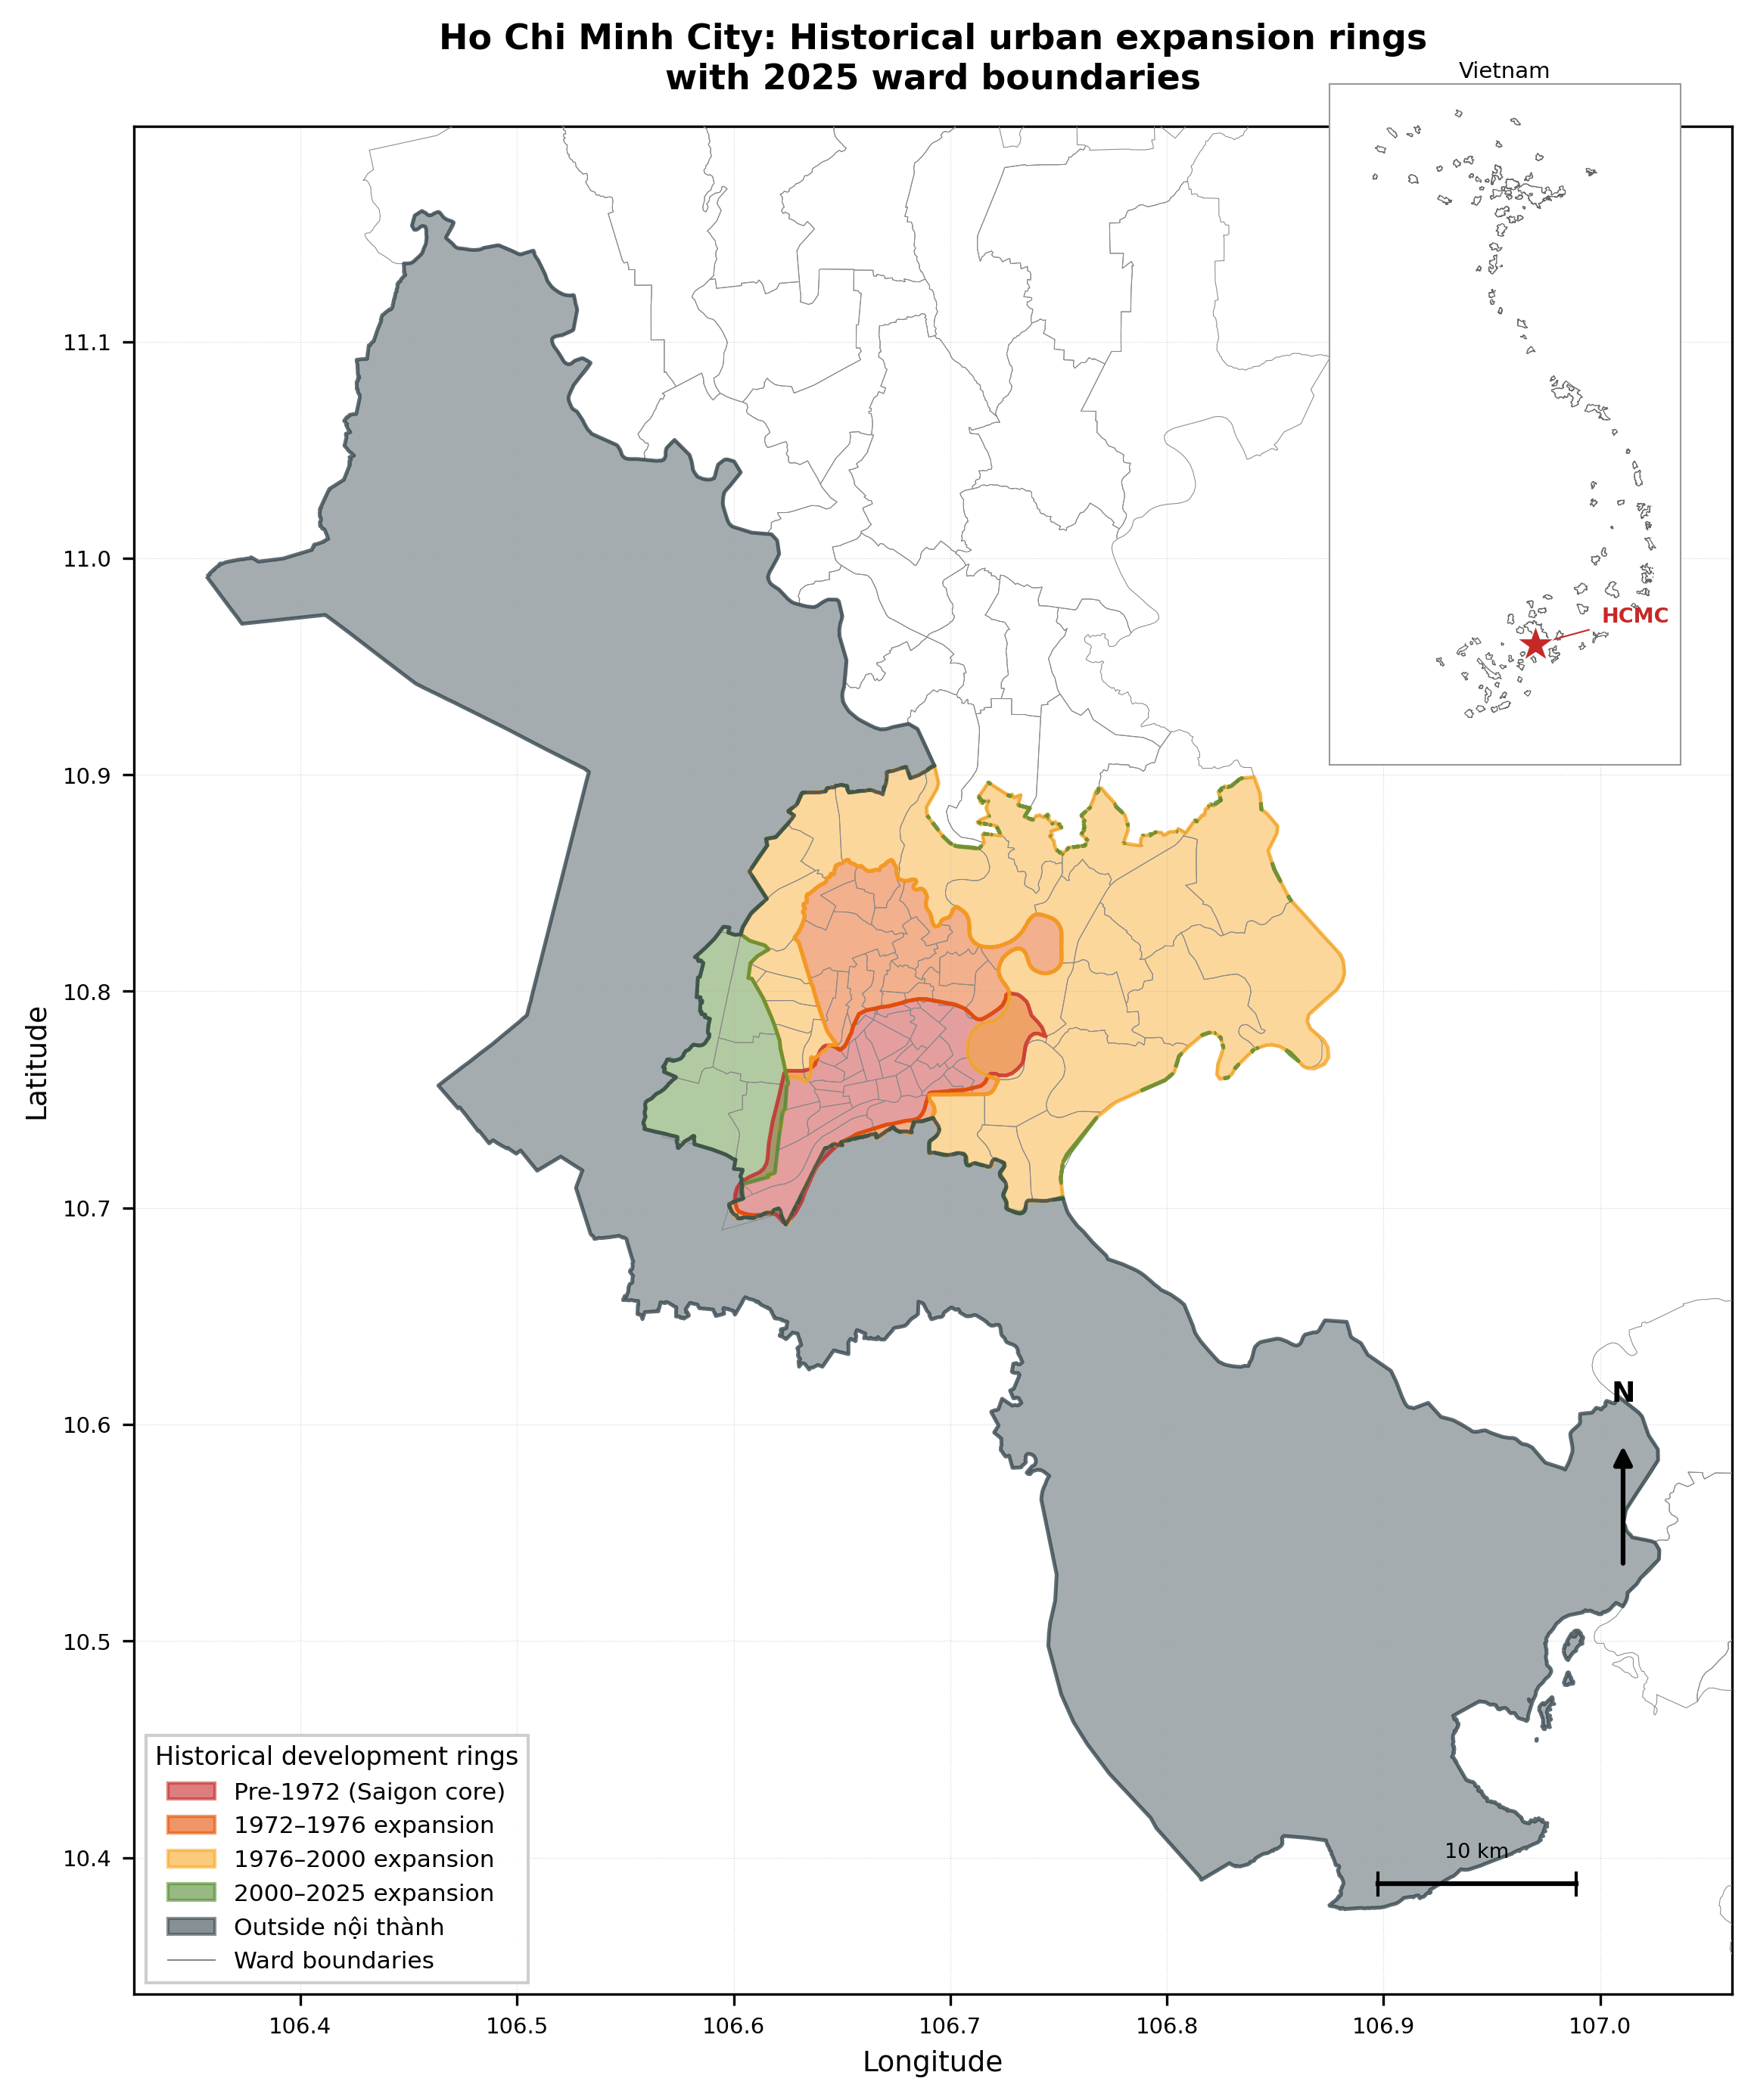
\includegraphics[width=0.8\textwidth]{../study_area_rings.png}
\caption{Study area and historical development rings of Ho Chi Minh City. The five concentric rings correspond to successive expansions of the \textit{nội thành} (inner city) boundary: pre-1972 Saigon core (71\,km$^2$), 1972--1976 war-era expansion (68\,km$^2$), 1976--2000 industrial expansion (316\,km$^2$), 2000--2025 market-era expansion (53\,km$^2$), and the outer peri-urban/rural zone. Ward boundaries shown in gray.}
\label{fig:studyarea}
\end{figure}

\begin{figure}[htbp]
\centering
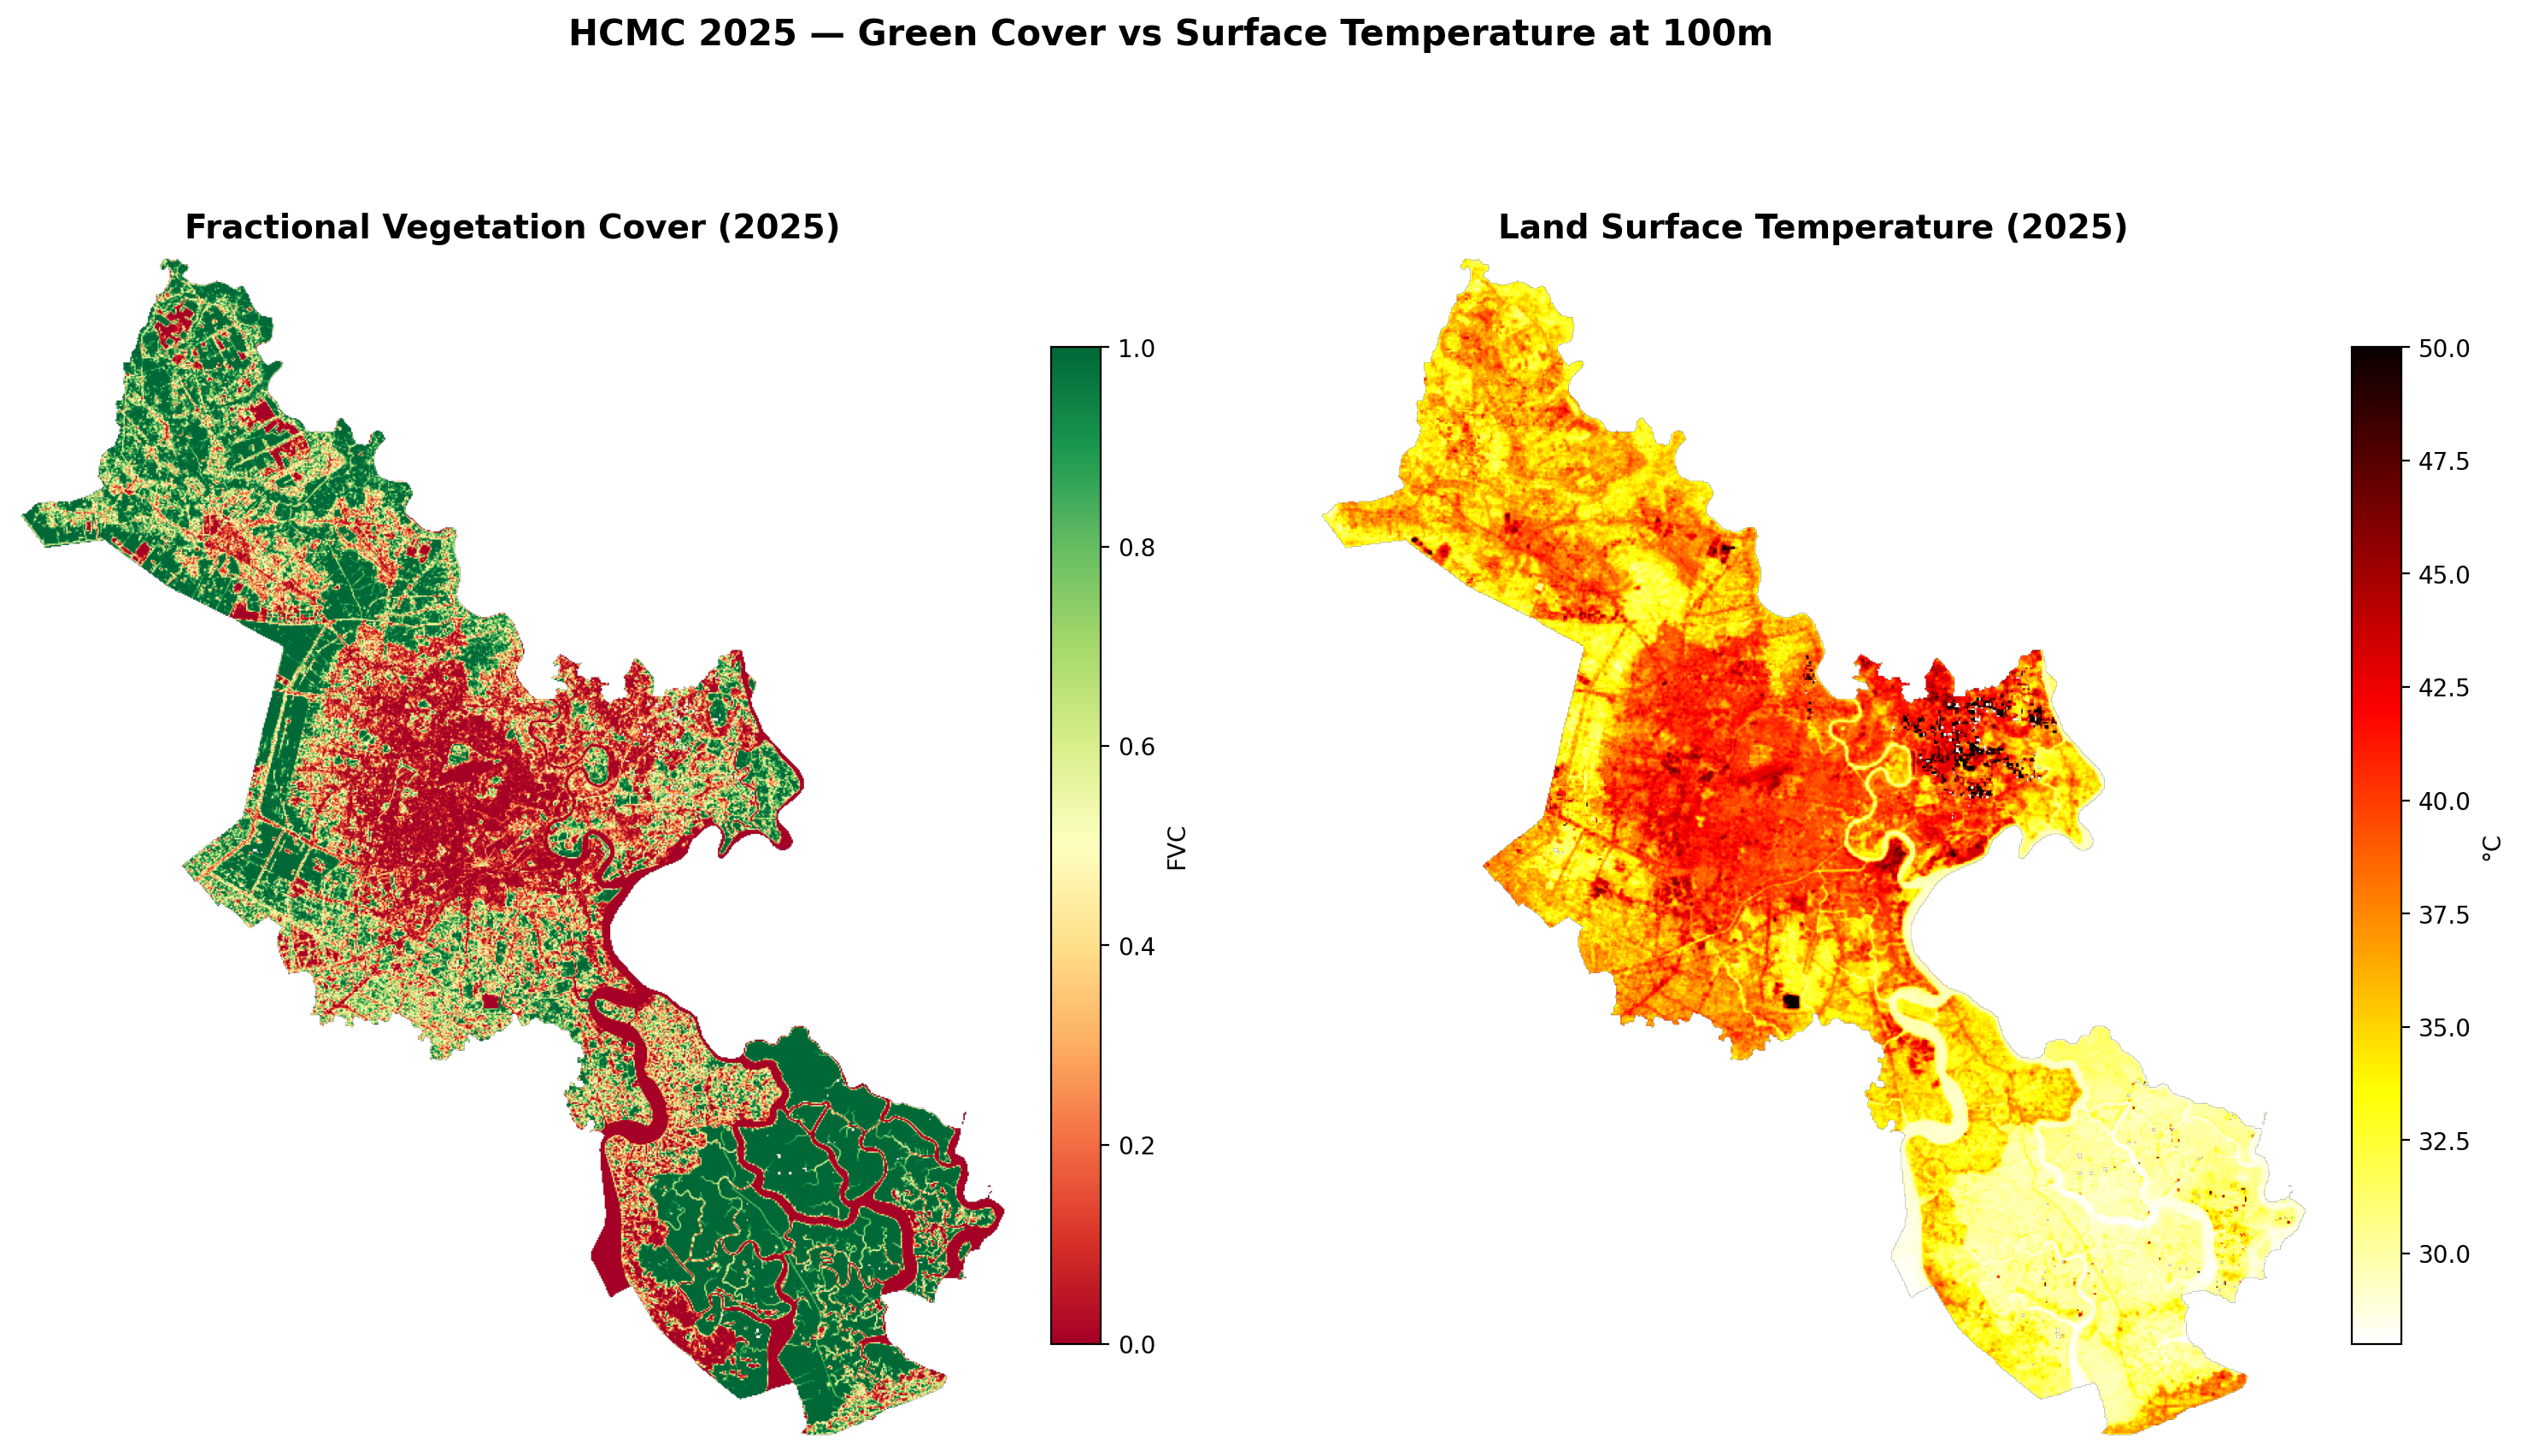
\includegraphics[width=\textwidth]{../eda_spatial_fvc_lst.png}
\caption{Spatial distribution of fractional vegetation cover (left) and land surface temperature (right) across Ho Chi Minh City at 100\,m resolution, 2024--2025. FVC derived from Sentinel-2 NDVI $\geq 0.4$ aggregated from 10\,m; LST from Landsat 8/9 thermal band. The contiguous high-LST, low-FVC zone in the city center corresponds to the pre-1972 and war-era development rings.}
\label{fig:spatial}
\end{figure}

\begin{figure}[htbp]
\centering
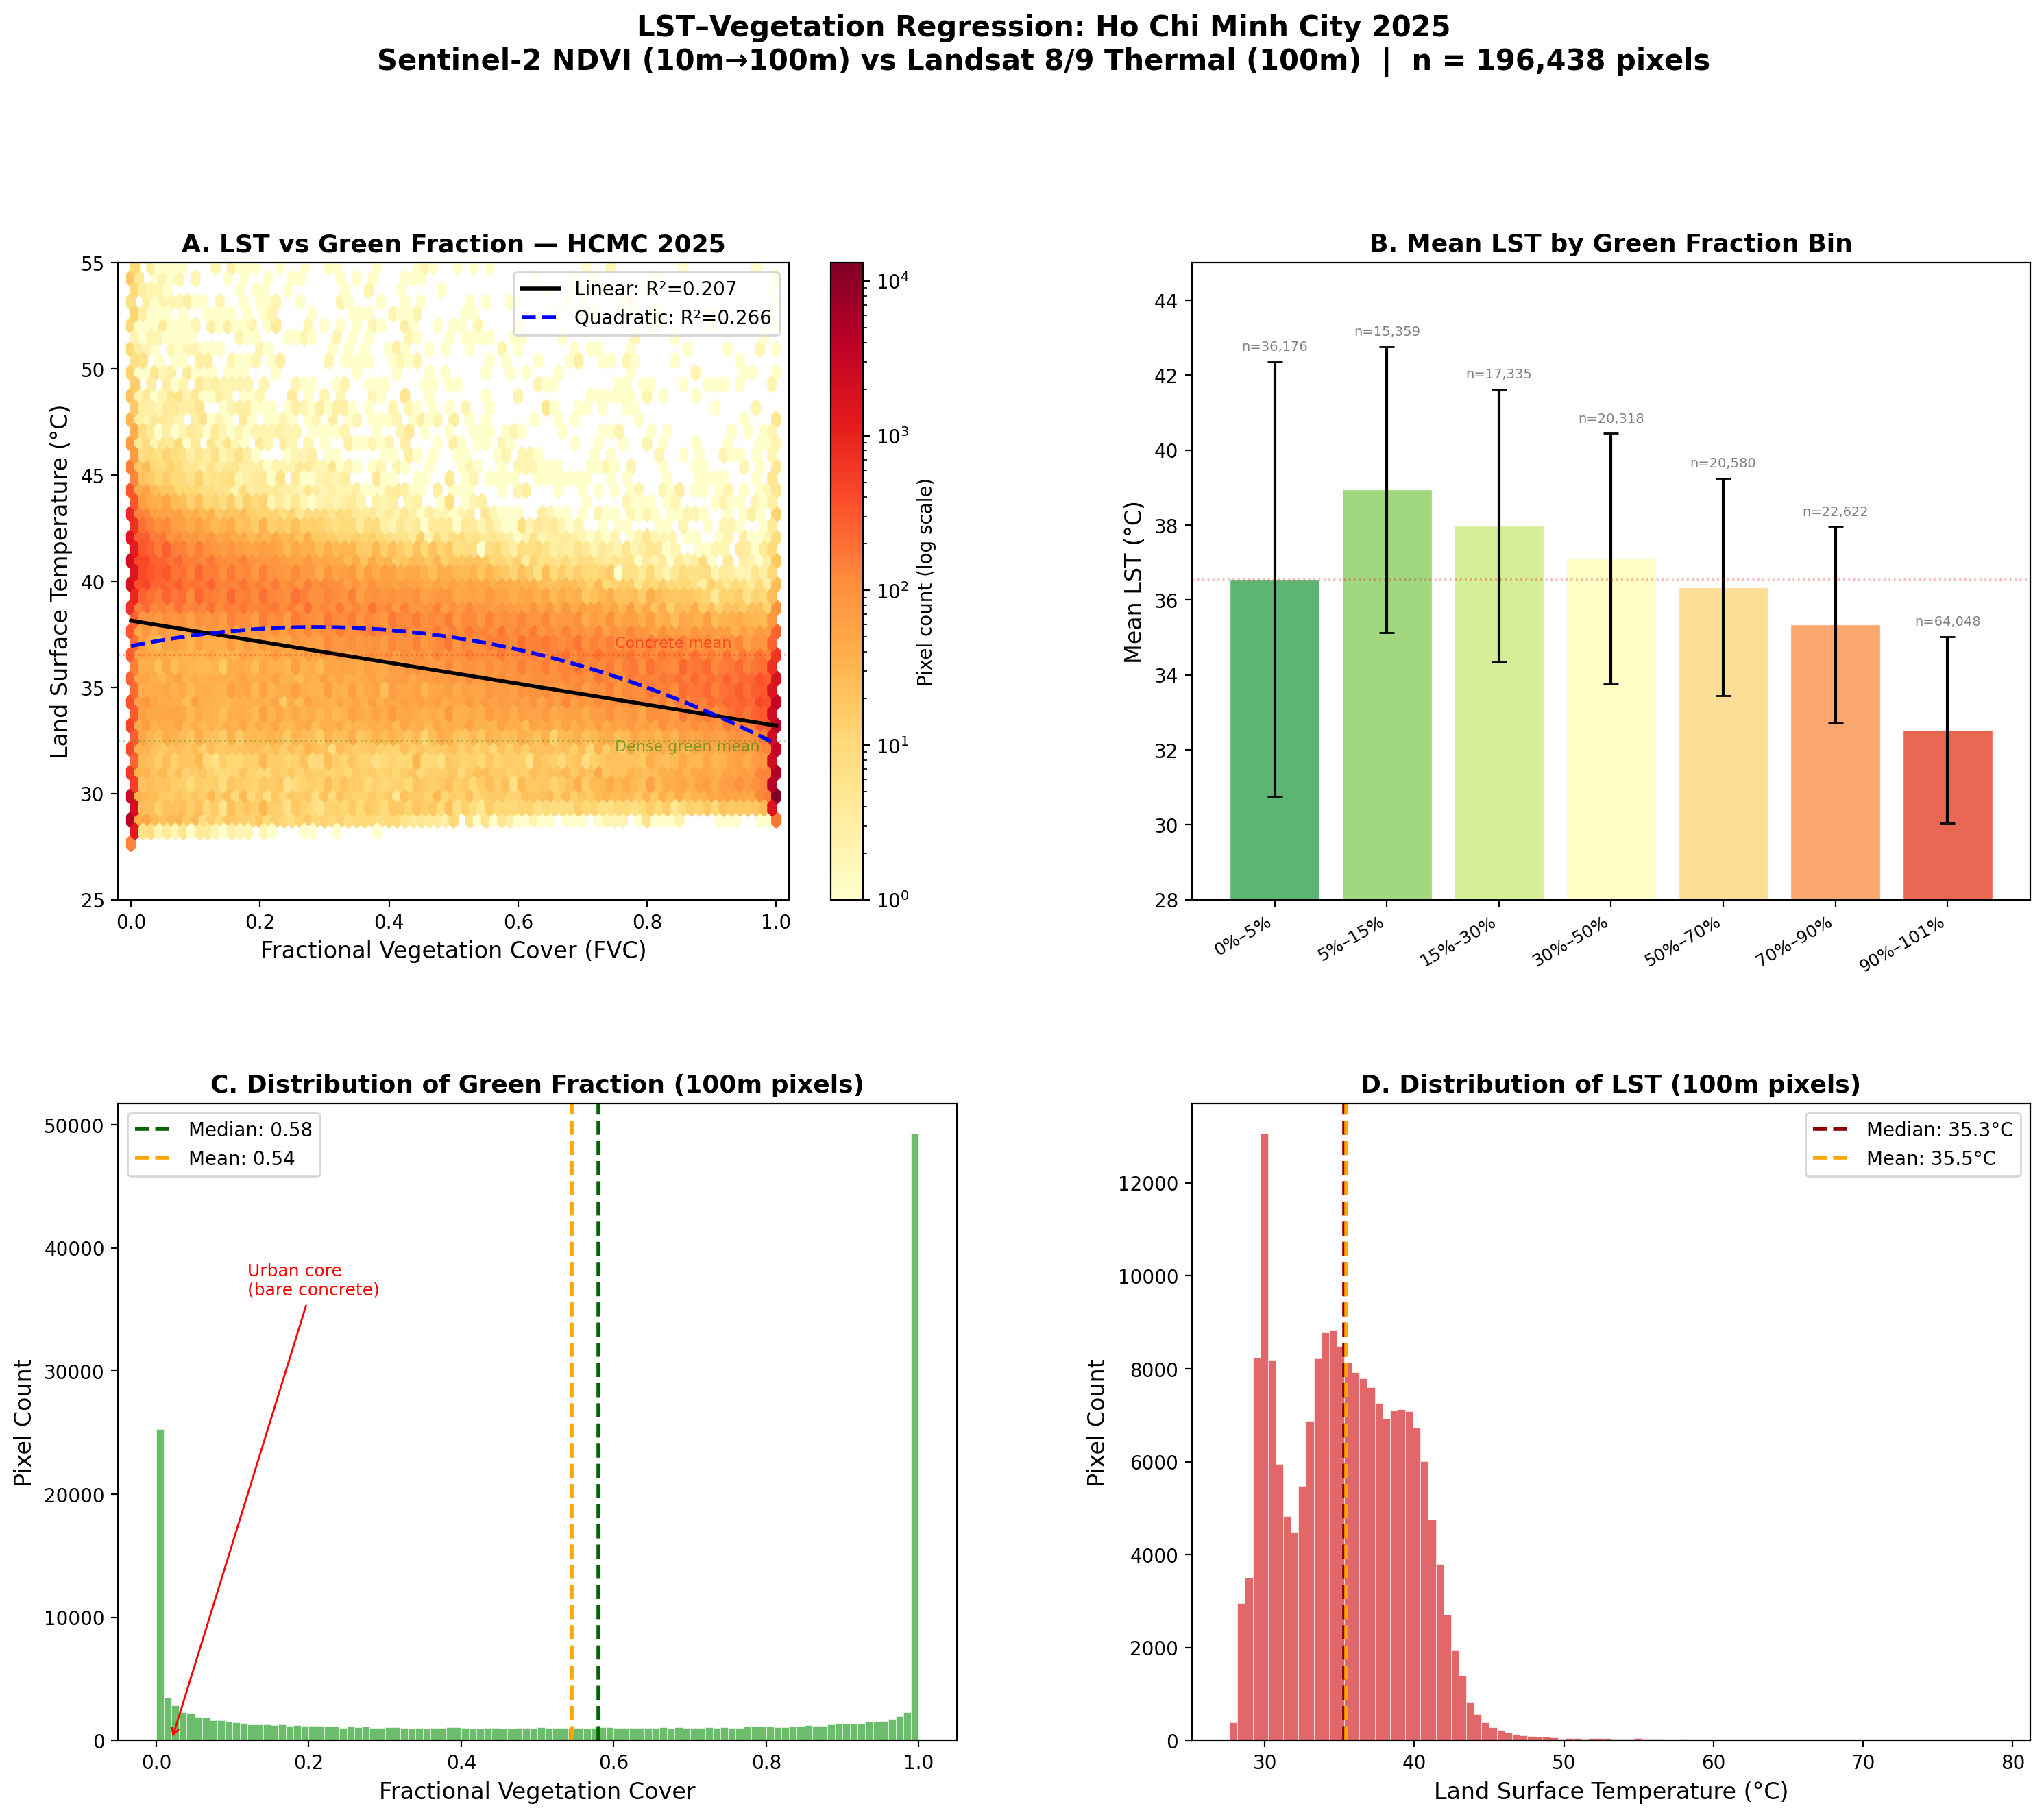
\includegraphics[width=\textwidth]{../eda_lst_fvc_regression.png}
\caption{LST--FVC regression analysis. (A) Density scatter plot with linear and quadratic fits. (B) Mean LST by FVC bin with standard deviation error bars. (C) Distribution of FVC across 196,438 pixels at 100\,m. (D) Distribution of LST. Note the bimodal FVC distribution (Panel C), reflecting the polarized landscape of dense urban core and vegetated periphery.}
\label{fig:scatter}
\end{figure}

\begin{figure}[htbp]
\centering
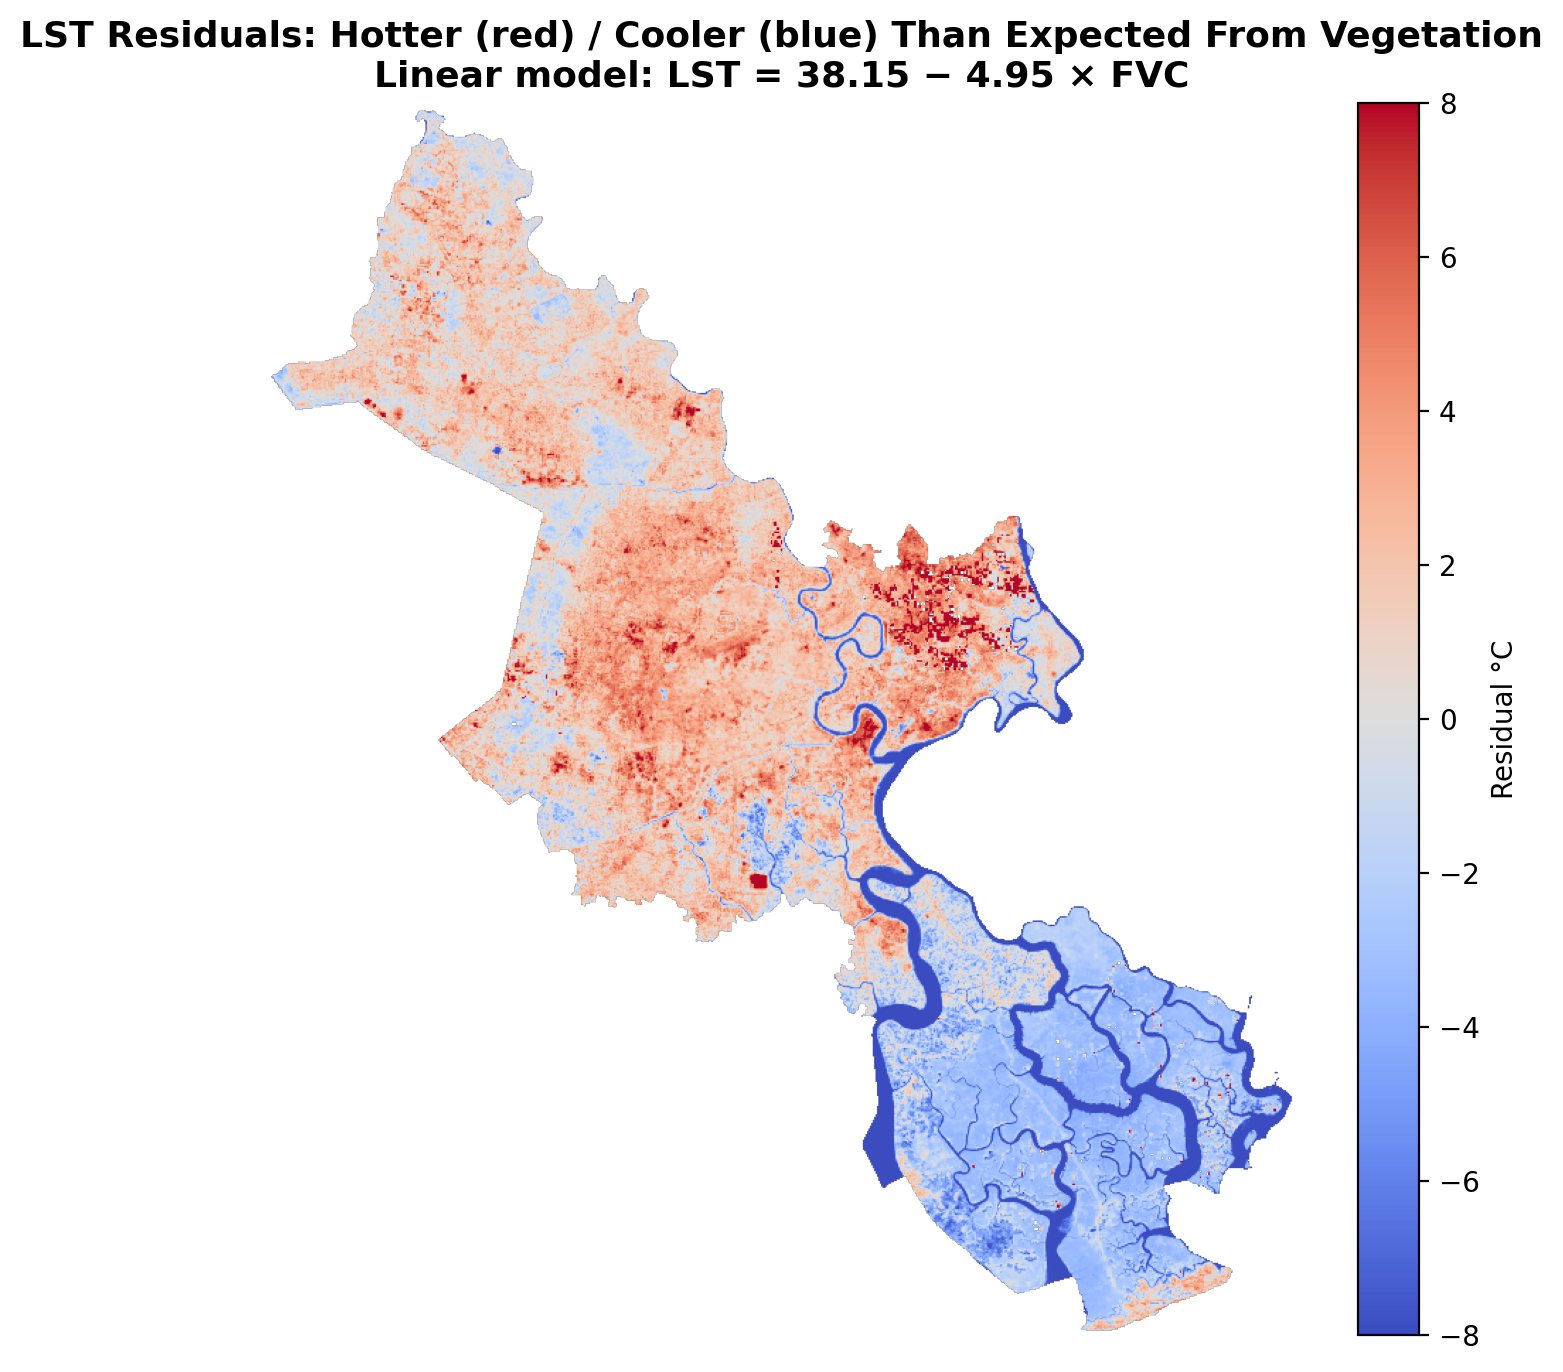
\includegraphics[width=0.8\textwidth]{../eda_lst_residual_map.png}
\caption{Spatial distribution of linear model residuals. Red indicates surfaces hotter than predicted by vegetation alone; blue indicates cooler. Positive residuals cluster in dense commercial/industrial zones (notably the Cát Lái port complex); negative residuals along waterways and in the Cần Giờ mangrove reserve. The strong spatial structure in residuals (Moran's $I = 0.654$) indicates that confounders such as urban morphology and water proximity are spatially clustered.}
\label{fig:residual}
\end{figure}

\begin{figure}[htbp]
\centering
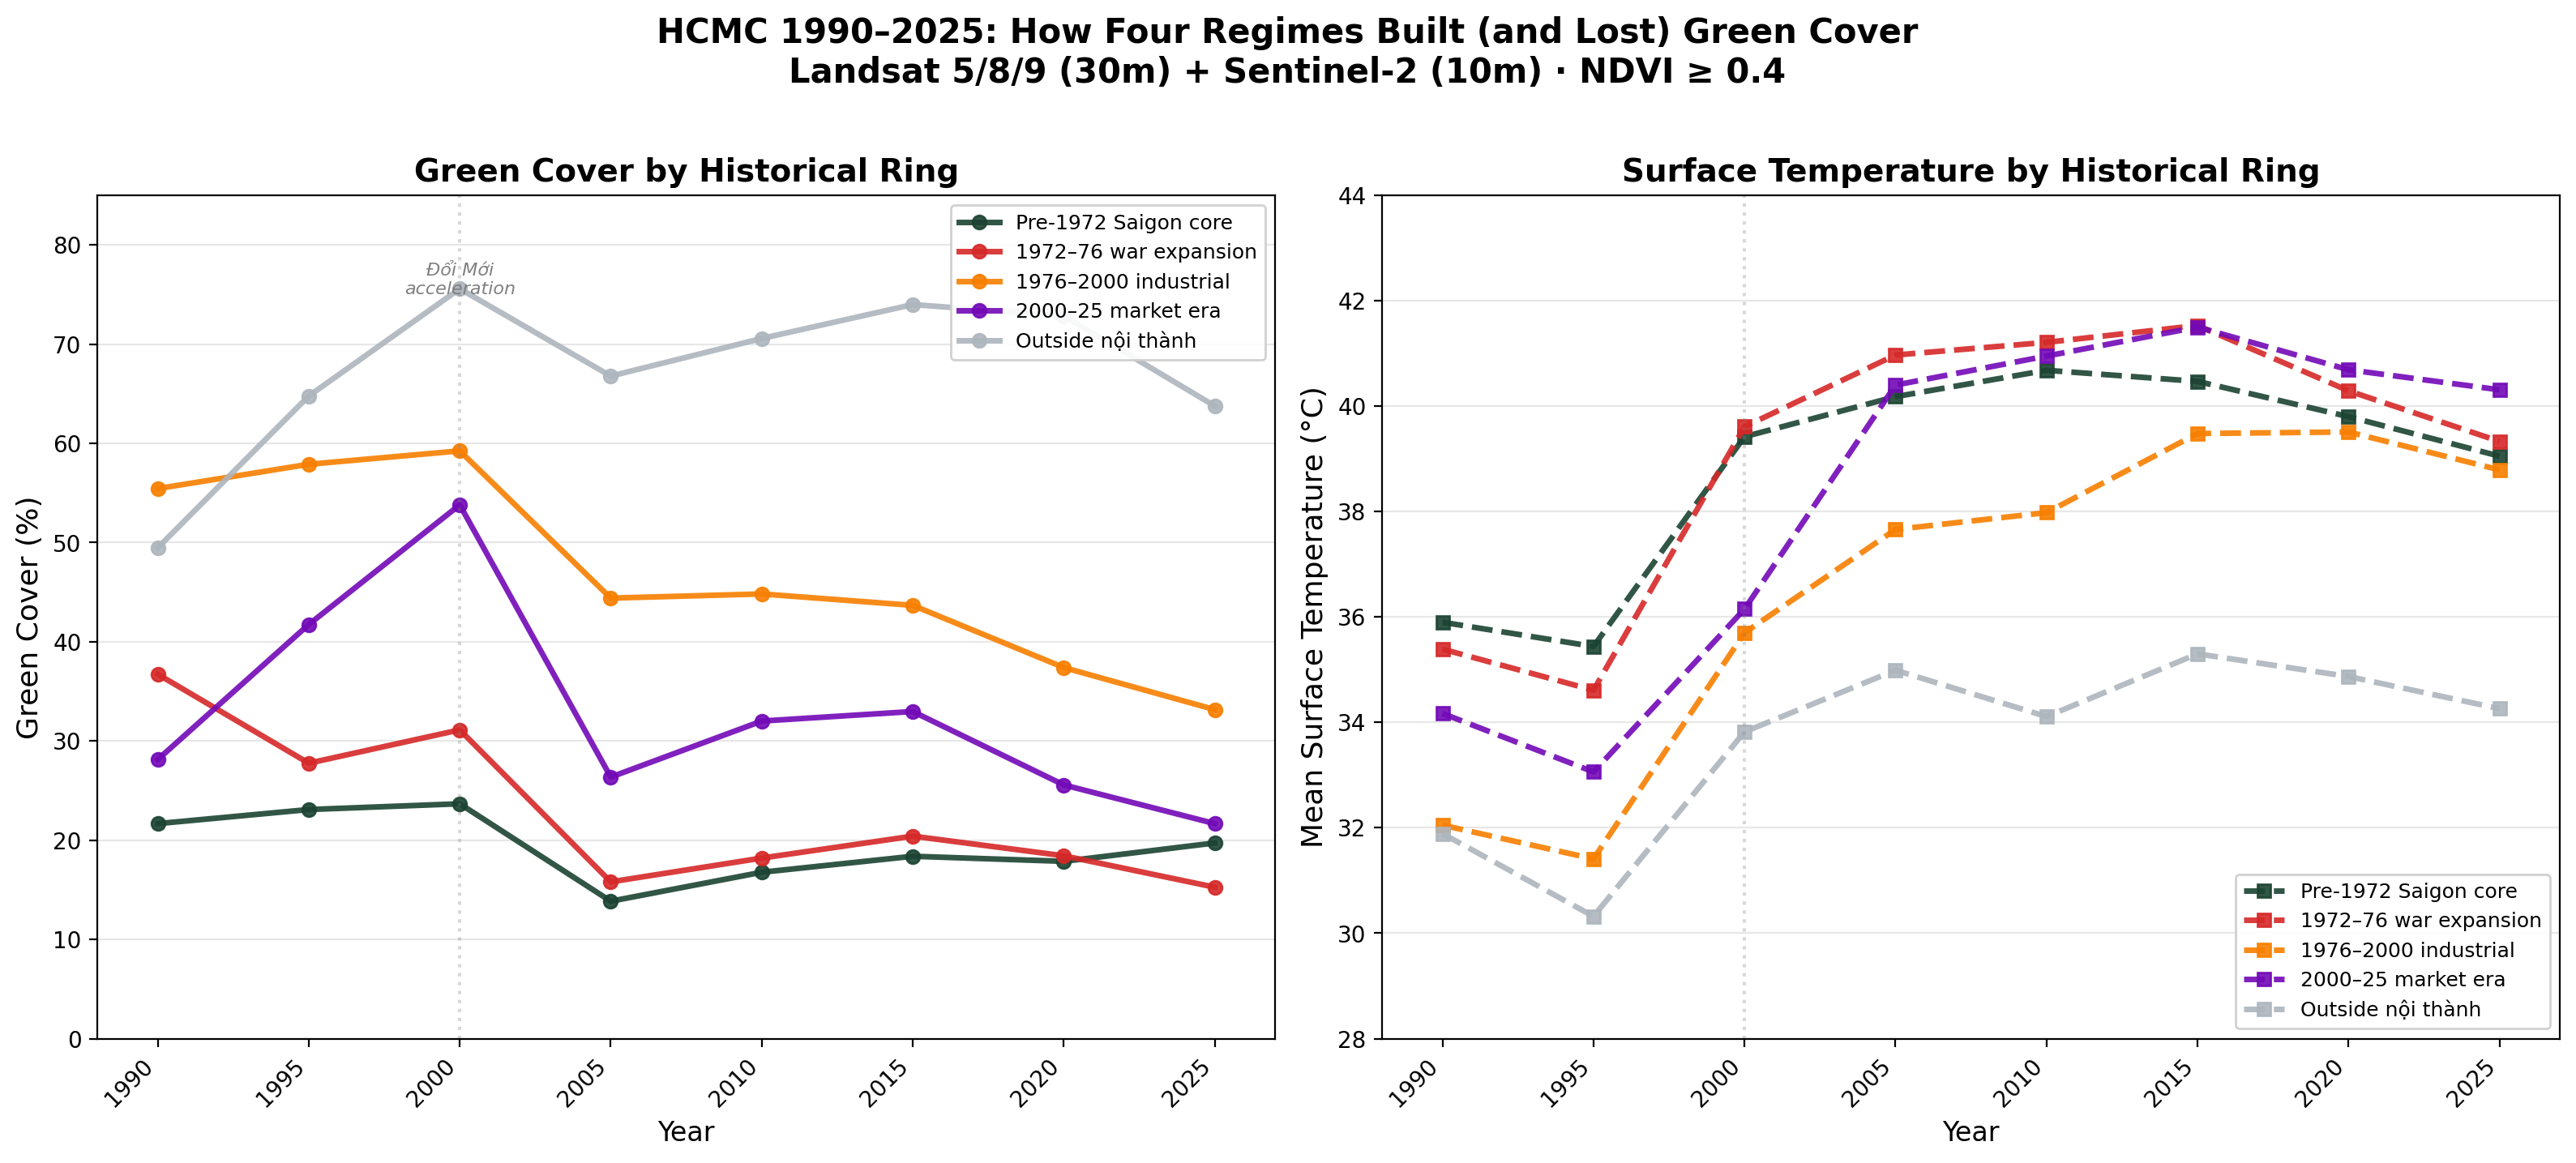
\includegraphics[width=\textwidth]{../temporal_green_lst_rings.png}
\caption{Green cover (left) and land surface temperature (right) by historical development ring, 1990--2025. Data for 1990--2020 from Landsat 5/8/9 at 30\,m; 2025 from Sentinel-2 at 10\,m (open markers). All inner rings show declining green cover and rising LST, with the war-era (1972--1976) and industrial (1976--2000) rings exhibiting the steepest losses. The sharp decline between 2000 and 2005 coincides with the post-Đổi Mới construction acceleration.}
\label{fig:temporal}
\end{figure}

\begin{figure}[htbp]
\centering
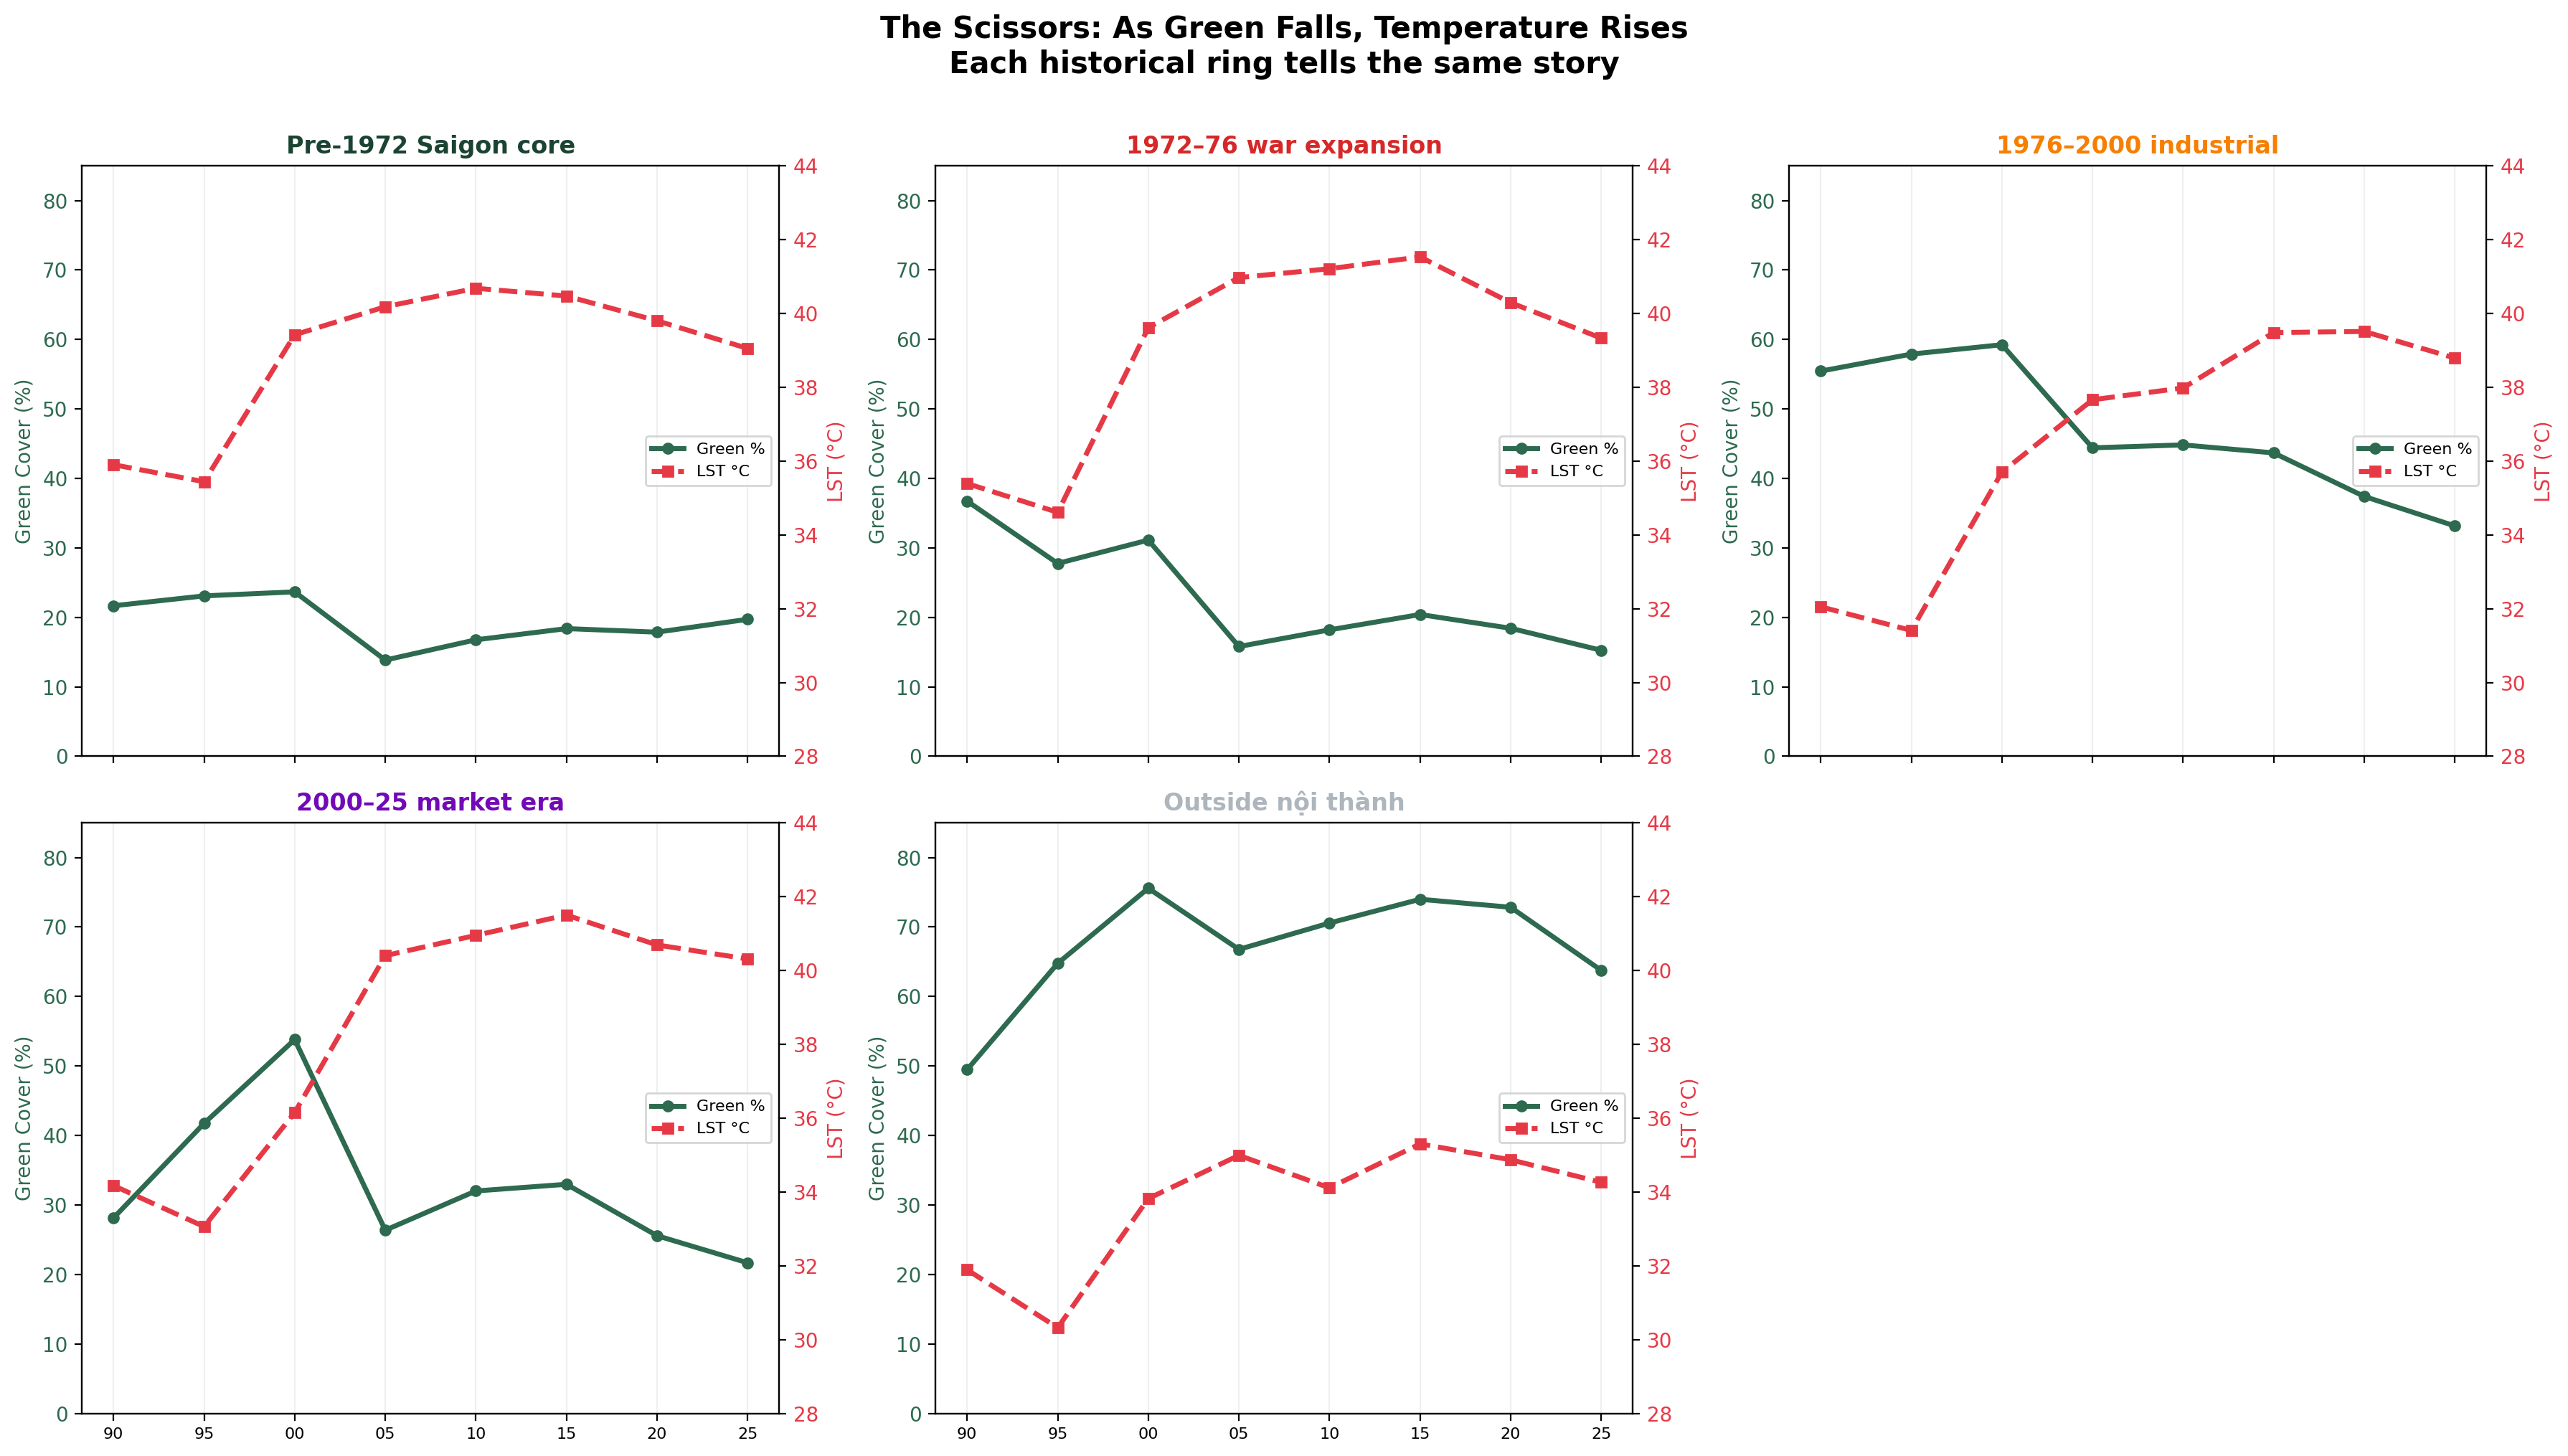
\includegraphics[width=\textwidth]{../temporal_scissors_by_ring.png}
\caption{The ``scissors'' pattern: green cover (solid, left axis) and surface temperature (dashed, right axis) for each historical development ring. As vegetation declines, surface temperature rises---a pattern consistent across all five rings, confirming that the LST--FVC relationship holds both spatially (cross-sectional regression) and temporally (within-ring trends).}
\label{fig:scissors}
\end{figure}

\begin{figure}[htbp]
\centering
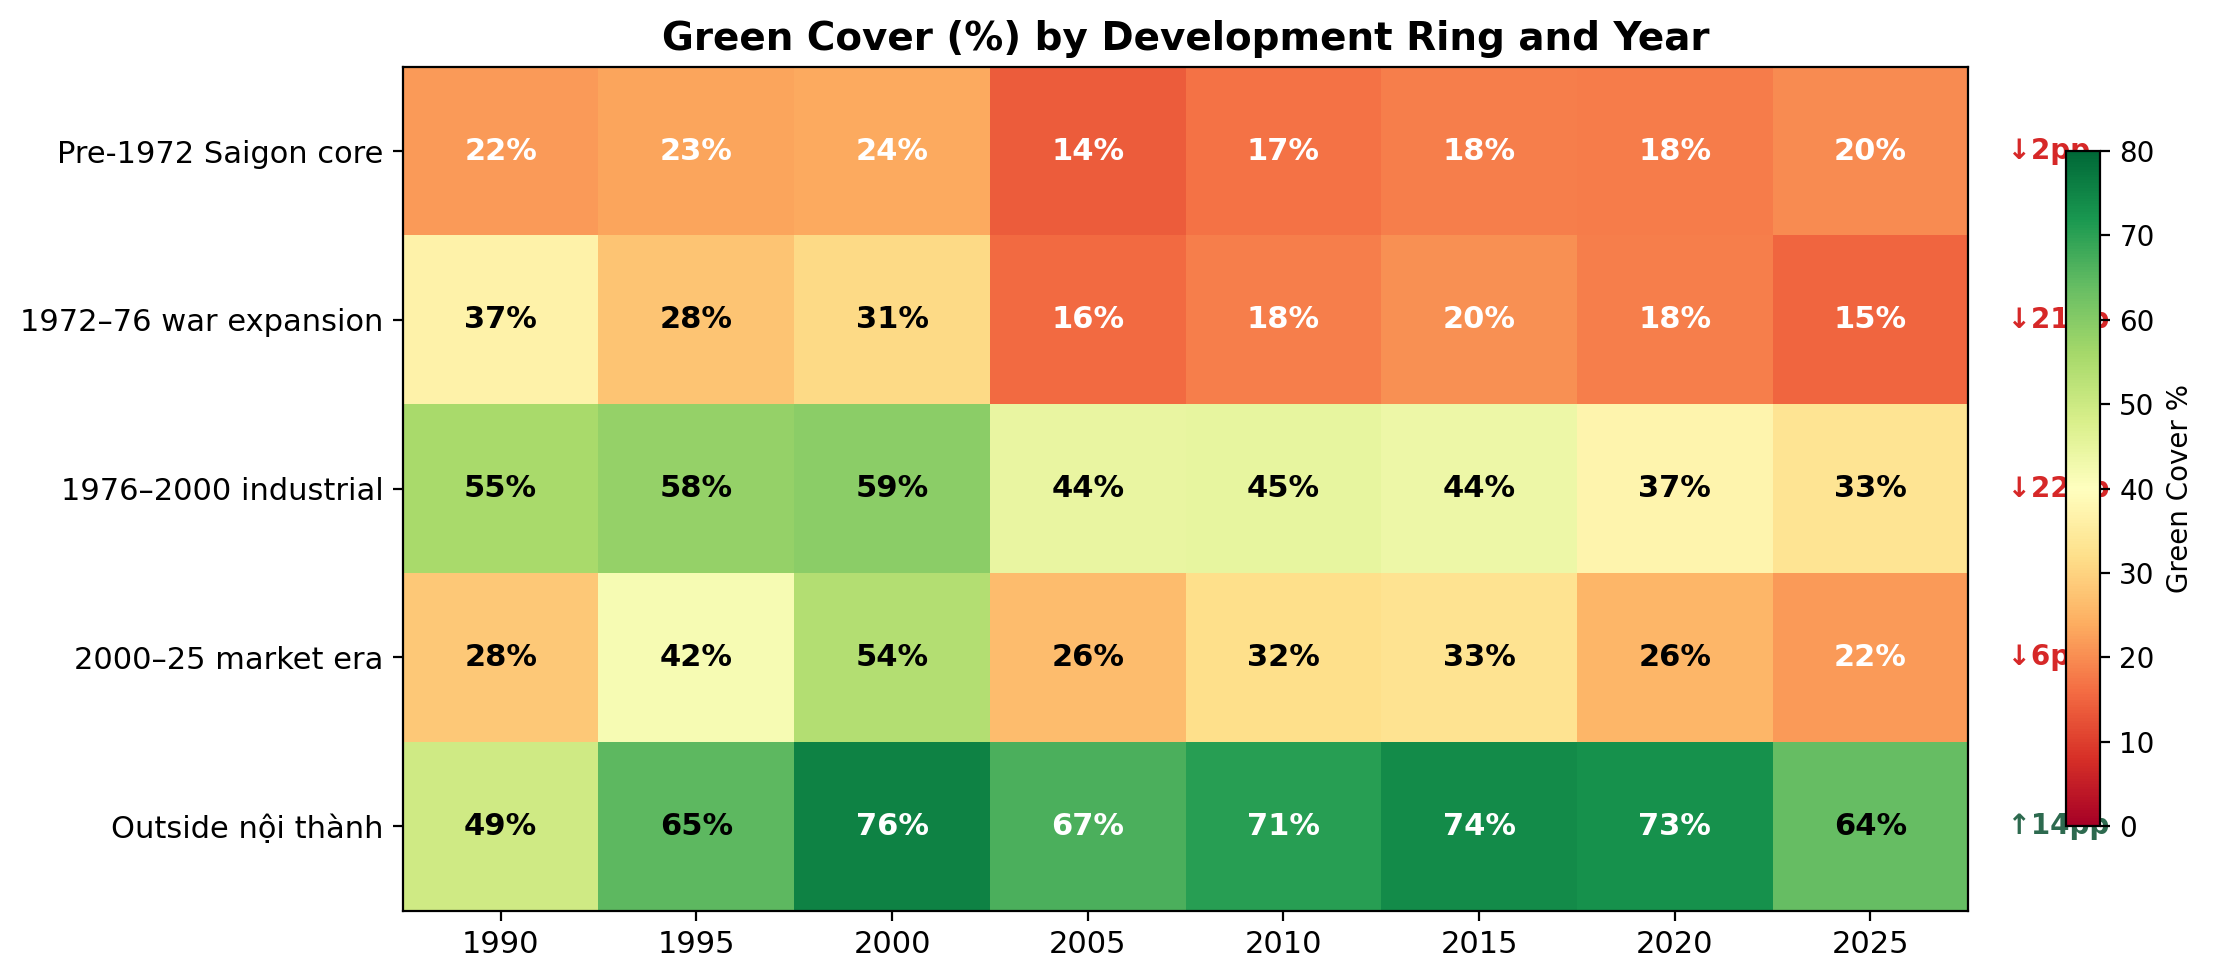
\includegraphics[width=\textwidth]{../temporal_heatmap_table.png}
\caption{Green cover (\%) by development ring and year, with net change in percentage points. The 1976--2000 industrial ring and the war-era ring each lost 18 pp within the Landsat-consistent period (1990--2020). The pre-1972 core---already largely concrete by 1990---showed the smallest absolute change. See Table~\ref{tab:temporal} for exact values and cross-sensor caveats.}
\label{fig:heatmap}
\end{figure}

\begin{figure}[htbp]
\centering
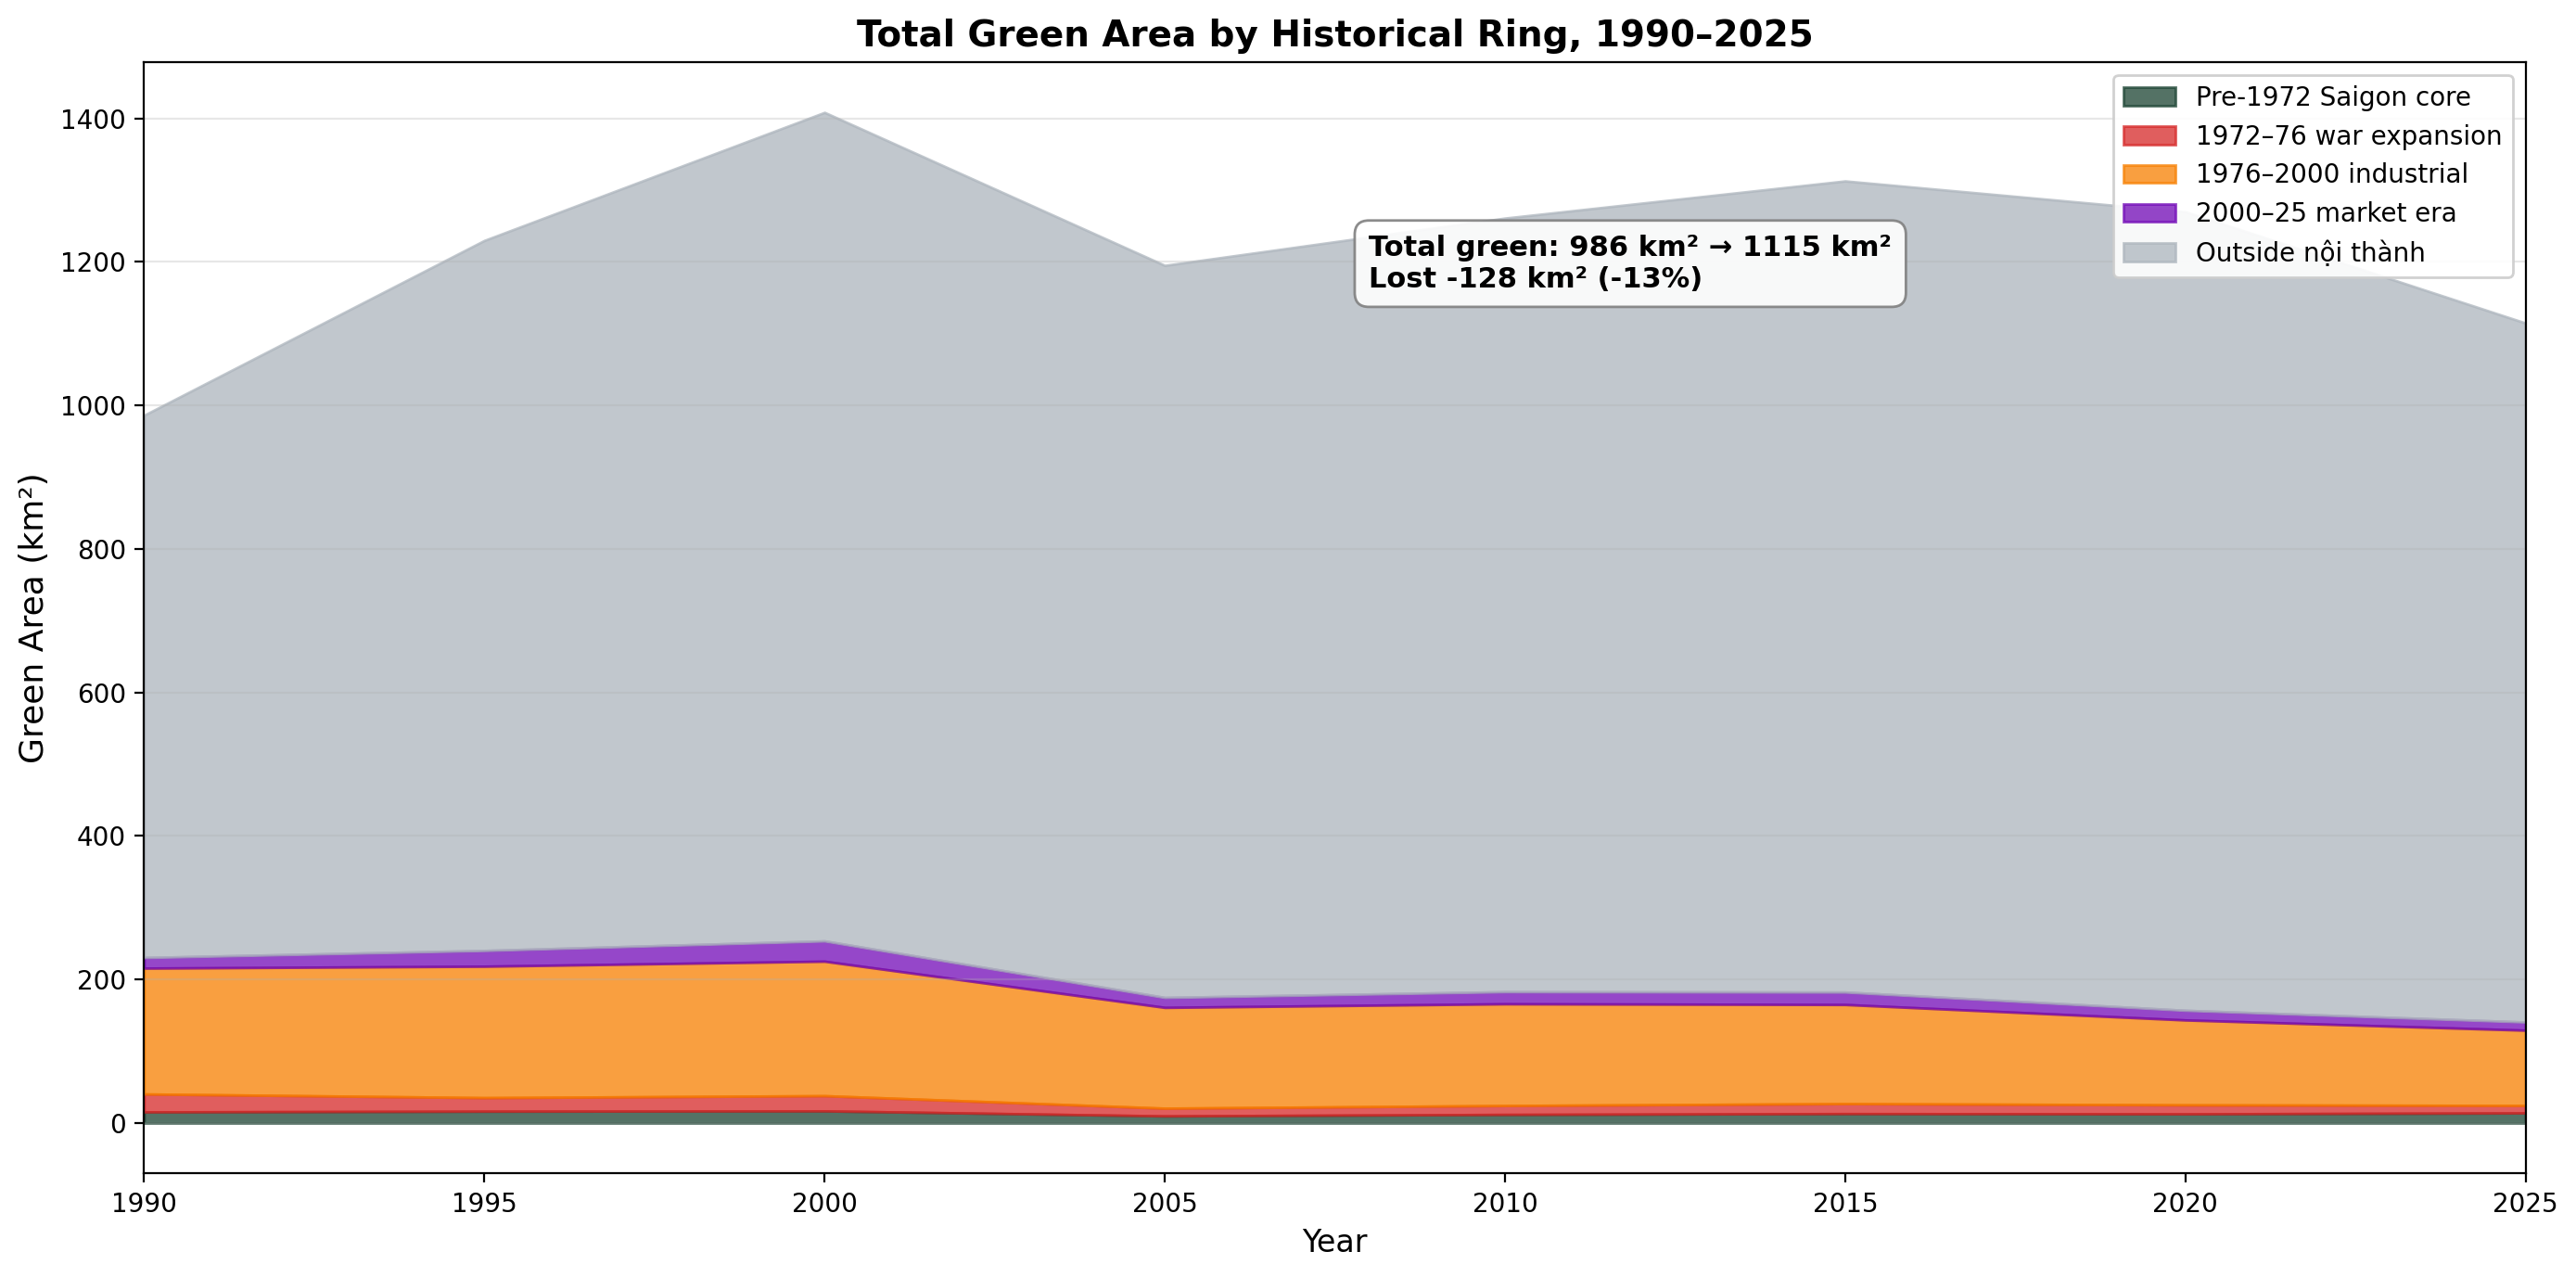
\includegraphics[width=\textwidth]{../temporal_stacked_green_area.png}
\caption{Total green area (km$^2$) by historical ring, 1990--2025. HCMC's green area peaked around 2000 at approximately 1,360\,km$^2$ before declining 10\% to approximately 1,230\,km$^2$ by 2020. The outer ring dominates total area, but the inner rings---where population density is highest---experienced the steepest proportional losses.}
\label{fig:stacked}
\end{figure}

\end{document}
